%==============================================================================
% ETHASL - Template for student projects at the ASL
% 2013.10: Péter Fankhauser
% This template is based on the IMRT Latex template by Eric A. Mueller.
%==============================================================================

\documentclass[10pt,twoside,a4paper]{report}

\usepackage{pdfpages}

% ETHASL package
% TODO Choose options according to your project
% som/bt/st/mt: Studies on Mechatronics, Bachelor Thesis, Semester Thesis, Master Thesis
% fs/hs: Spring term, Autumn term
% german/english: German/English
\usepackage[mt,hs,english]{packages/ethasl}
% Activate for german language
%\usepackage{german}
%\usepackage{ae}
%%%%%%%%%%%%%%%%%%%%%%%%%%%%%%%%%%%%%%%%%%%%%%%%%%%%%%%%%%%%%%%%%%%%%%%%%%%%%%%
% LaTeX preamble
%%%%%%%%%%%%%%%%%%%%%%%%%%%%%%%%%%%%%%%%%%%%%%%%%%%%%%%%%%%%%%%%%%%%%%%%%%%%%%%
% Encoding settings
\usepackage[utf8]{inputenc}
\usepackage[OT1]{fontenc}

% Paper size
\usepackage{a4}

% Headings
\usepackage{fancyhdr}

% More symbols
\usepackage{textcomp}\usepackage{gensymb}

% Math support for Times font
%\usepackage{txfonts}

% ISO date
\usepackage[english]{isodate}

% Multi column
\usepackage{multicol}

% Figures
\usepackage{graphicx}

% Subfigures (obsolete)
\usepackage{subfigure}

% Bibliography
\usepackage[numbers]{natbib}

% Nicer tables
\usepackage{booktabs}
\usepackage{array}
\usepackage{multirow}

% Colors
\usepackage{color}
\usepackage{colortbl}
\definecolor{black}{rgb}{0,0,0}
\definecolor{white}{rgb}{1,1,1}
\definecolor{darkred}{rgb}{0.5,0,0}
\definecolor{darkgreen}{rgb}{0,0.5,0}
\definecolor{darkblue}{rgb}{0,0,0.5}

% Additional math functionality
\usepackage{amsmath}
\usepackage{amssymb}

% Nice fractions
\usepackage{nicefrac}

% Upper case greek letters
\usepackage{upgreek}

% ISO math notation
\usepackage{isomath}
\renewcommand{\vec}{\vectorsym}
\newcommand{\mat}{\matrixsym}

% Units
\usepackage{units}

% Rotated objects
\usepackage{rotating}

% Indent
\setlength{\parindent}{0em}

% Include PDF pages
\usepackage{pdfpages}
\includepdfset{pages={-}, frame=true, pagecommand={\thispagestyle{fancy}}}

% Headings
\rhead[\thepage]{\nouppercase{\rightmark}}
\lhead[\nouppercase{\leftmark}]{\thepage}
\cfoot{}

% Gantt chart
\usepackage{pgfgantt}

% Links (last package)
\PassOptionsToPackage{hyphens}{url}\usepackage{hyperref}

% Clever references (has to be loaded after hyperref)
\usepackage{cleveref}

\usepackage{mathrsfs}
\usepackage{bm}
%%%%%%%%%%%%%%%%%%%%%%%%%%%%%%%%%%%%%%%%%%%%%%%%%%%%%%%%%%%%%%%%%%%%%%%%%%%%%%%
% Title page
% %%%%%%%%%%%%%%%%%%%%%%%%%%%%%%%%%%%%%%%%%%%%%%%%%%%%%%%%%%%%%%%%%%%%%%%%%%%%%%%
\begin{document}

% % TODO Add your title
\title{Use of a DVS for High Speed Applications}
% \subtitle{bla bla bla}

\studentA{Weizhen Huang}

\supervisionA{Florian Tschopp} \supervisionB{Ignacio Alzugaray}

\projectYear{\the\year} % This year
% \projectYear{\advance\year by -1 \the\year\advance\year by
% 1} % Last year

\maketitle
\pagestyle{plain} \pagenumbering{roman}

%%%%%%%%%%%%%%%%%%%%%%%%%%%%%%%%%%%%%%%%%%%%%%%%%%%%%%%%%%%%%%%%%%%%%%%%%%%%%%%
% Declaration of originality
%%%%%%%%%%%%%%%%%%%%%%%%%%%%%%%%%%%%%%%%%%%%%%%%%%%%%%%%%%%%%%%%%%%%%%%%%%%%%%%
\pagestyle{empty}
% TODO Modify placeholders in declaration.tex
% % TODO Add title, student first/last name, supervisor first/last name.

\section*{Declaration of Originality}

\vspace{1cm}

I hereby declare that the written work I have submitted entitled

\vspace{0.5cm}

% TODO Add title
\textbf{Use of a DVS for High Speed Applications}

\vspace{0.5cm}

is original work which I alone have authored and which is written in
my own words.\footnote{Co-authored work: The signatures of all authors
  are required. Each signature attests to the originality of the
  entire piece of written work in its final form.}

\vspace{1cm}

\textbf{Author}

\vspace{0.5cm}

\begin{tabular}{ p{5cm} p{5cm} }
  Weizhen & Huang \\
\end{tabular}

\vspace{0.5cm}

\textbf{Student supervisors}

\vspace{0.5cm}

\begin{tabular}{ p{5cm} p{5cm} }
  Florian& Tschopp\\
  Ignacio& Alzugaray\\
\end{tabular}

\vspace{0.5cm}

\textbf{Supervising lecturer}

\vspace{0.5cm}

\begin{tabular}{ p{5cm} p{5cm} }
  Roland & Siegwart \\
\end{tabular}

\vspace{1cm}

With the signature I declare that I have been informed regarding
normal academic citation rules and that I have read and understood the
information on 'Citation etiquette'
(\url{https://www.ethz.ch/content/dam/ethz/main/education/rechtliches-abschluesse/leistungskontrollen/plagiarism-citationetiquette.pdf}).
The citation conventions usual to the discipline in question here have
been respected.

\vspace{0.5cm}

The above written work may be tested electronically for plagiarism.

\vspace{4cm}

\begin{tabular}{ p{5cm} p{1cm} p{5cm} }
  \cline{1-1} \cline{3-3}
  Place and date & & Signature \\
\end{tabular}

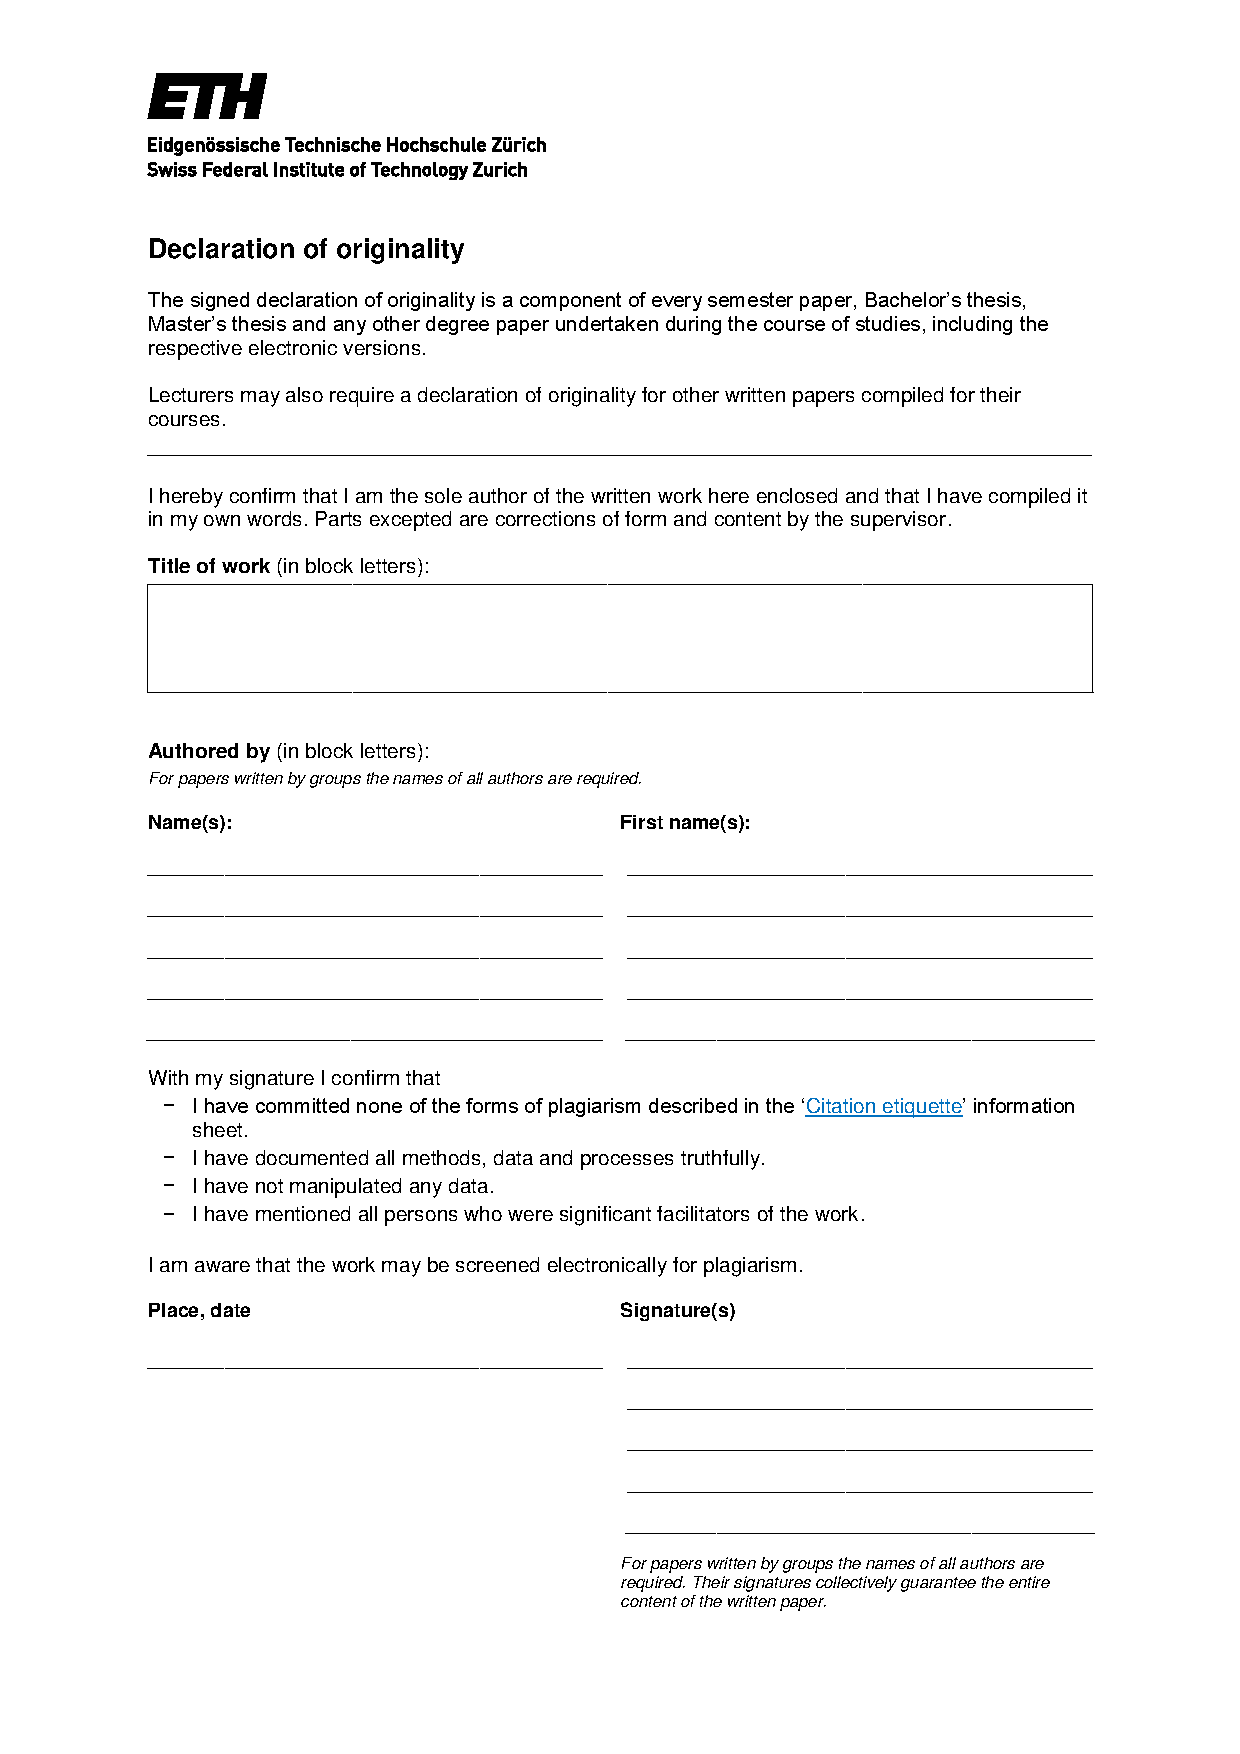
\includepdf[pagecommand={}]{chapters/declaration-originality.pdf}


%%%%%%%%%%%%%%%%%%%%%%%%%%%%%%%%%%%%%%%%%%%%%%%%%%%%%%%%%%%%%%%%%%%%%%%%%%%%%%%
% Table on contents
%%%%%%%%%%%%%%%%%%%%%%%%%%%%%%%%%%%%%%%%%%%%%%%%%%%%%%%%%%%%%%%%%%%%%%%%%%%%%%%

% Table of Contents depth (TODO change if necessary)
\setcounter{tocdepth}{2}

\tableofcontents
\cleardoublepage

%%%%%%%%%%%%%%%%%%%%%%%%%%%%%%%%%%%%%%%%%%%%%%%%%%%%%%%%%%%%%%%%%%%%%%%%%%%%%%%
% Chapters standard
%%%%%%%%%%%%%%%%%%%%%%%%%%%%%%%%%%%%%%%%%%%%%%%%%%%%%%%%%%%%%%%%%%%%%%%%%%%%%%%
\chapter*{Preface}
\addcontentsline{toc}{chapter}{Preface}
%\chapter*{Vorwort}
%\addcontentsline{toc}{chapter}{Vorwort}

Bla bla \dots \cleardoublepage \chapter*{Abstract}
\addcontentsline{toc}{chapter}{Abstract} Event cameras are
bio-inspired cameras that capture pixel-level intensity changes at a
rate of up to \SI{1}{\mega\hertz}. They naturally respond to edges in
the scene and are free from motion blur.

We propose a method which performs SLAM in planar scenes and 6-DoF
motion estimation in unstructured scenes with a monocular event
camera, no additional sensing. This method is based on a contrast
maximization pipeline. Events are grouped by a small temporal window
and warped with the optimal motion parameters that produce the
sharpest image. When performing SLAM, all the images are tracked using
image-to-model alignment, but only a selective set of keyframes are
used to construct the map. This method performs favorably against the
ground truth, and is able to track high speed motions.

\cleardoublepage \chapter*{Symbols}
\label{sec:symbols}
\addcontentsline{toc}{chapter}{Symbols}
%\chapter*{Symbolverzeichnis}
%\label{sec:symbole}
%\addcontentsline{toc}{chapter}{Symbolverzeichnis}

\section*{Symbols}
% \section*{Symbole}

\begin{tabbing}
  \hspace*{1.6cm} \= \kill
  $\mat{I}_n$    \> $n\times n$ identity matrix \\[0.5ex]
  $\mat{K}$      \> camera projection matrix \\[0.5ex]
  $\mat{A}^\top$  \> matrix transpose \\[0.5ex]
  $\mat{A}^{-1}$			 \> matrix inverse \\[0.5ex]
  $\vec{0}_{m\times n}$     \> an $m\times n$-vector whose entries are 0 \\[0.5ex]
  $\mathbb{R}^n$     \> space of real $n$-vectors, $n$-dimensional Euclidean space	\\[0.5ex]
  $\mathbb{S}^n$     \> $n$-sphere	\\[0.5ex]
  $SO(3)$     \> 3D special orthogonal group, 3D rotation group	\\[0.5ex]
  $\mathfrak{so}(3)$  \> the vector space of $3\times3$ skew-symmetric matrices \\[0.5ex]
  $SE(3)$     \> 3D special Euclidean group, the group of rigid body motion\\[0.5ex]
  $e$                     \> event \\[0.5ex]
  $p$                     \> event polarity\\[0.5ex]
  $\mathscr{{E}}$                     \> a set of events\\[0.5ex]
  $\delta$                     \> Dirac delta\\[0.5ex]
  $\vec{x}$                     \> 2D pixel coordinate\\[0.5ex]
  $\bar{\vec{x}}$                     \> homogeneous coordinate\\[0.5ex]
  $\tilde{\vec{x}}$                     \> calibrated coordinate\\[0.5ex]
  $\vec{X}$                     \> 3D point in space\\[0.5ex]
  $\mat{R}$                     \> orientation\\[0.5ex]
  $\vec{t}$                     \> translation\\[0.5ex]
  $\vec{T}$                     \> camera pose, including $\mat{R}$ and $\vec{t}$  \\[0.5ex]
  $\bm{\omega}$                     \> angular velocity\\[0.5ex]
  $\vec{v}$                     \> linear velocity\\[0.5ex]
  $\vec{n}$                     \> normal direction of a plane\\[0.5ex]
  $\bm{\theta}$                     \> parameter set, might include $\mat{R},\vec{t},\bm{\omega},\vec{v}\text{ and }\vec{n}$ \\[0.5ex]
  $^\wedge$                     \> hat operator\\[0.5ex]
  $\sim$                     \> equality up to a non-zero scale\\[0.5ex]


  % \mathcal{I}(\vec{x})
\end{tabbing}

\section*{Acronyms and Abbreviations}
% \section*{Akronyme und Abkürzungen}
\begin{tabbing}
  \hspace*{1.6cm}  \= \kill
  DVS \> Dynamic Vision Sensor\\[0.5ex]
  APS \> Active Pixel Sensor \\[0.5ex]
  DoF \> Degrees of Freedom \\[0.5ex]
  SLAM \> Simultaneously Localizing and Mapping \\[0.5ex]
  BFGS \> Broyden-Fletcher-Goldfarb-Shanno Algorithm \\[0.5ex]
\end{tabbing}
 \cleardoublepage

%%%%%%%%%%%%%%%%%%%%%%%%%%%%%%%%%%%%%%%%%%%%%%%%%%%%%%%%%%%%%%%%%%%%%%%%%%%%%%%
% Chapters custom
%%%%%%%%%%%%%%%%%%%%%%%%%%%%%%%%%%%%%%%%%%%%%%%%%%%%%%%%%%%%%%%%%%%%%%%%%%%%%%%
\pagestyle{fancy} \pagenumbering{arabic}

% TODO Add your own chapters here
\chapter{Introduction}
\label{sec:introduction}
% \chapter{Einleitung}
% \label{sec:einleitung}

Frame-based cameras that widely used in computer vision output images
at a pre-set rate, even when the intensity values stay unchanged,
resulting in redundant data. When the scene moves too fast, an
insufficient frame rate would cause motion blur. To address this
problem, in 2008 \citet{lichtsteiner2008128} present an event-based
camera called DVS (dynamic vision sensor) that reports pixel-level log
intensity changes at a rate of \unit{MHz} scale. Unlike a traditional
camera that outputs a frame until all the pixels are scanned, the
event-based camera outputs are asynchronous: when the intensity change
at a pixel reaches a threshold
$\mid\ln{I(t)}-\ln{I(t-\Delta t)}\mid>C$, the sensor outputs an
``event'' $e=\{x,y,t,p\}$, which includes the pixel coordinate
$(x, y)$, the timestamp $t$ and the polarity $p=\pm1$ indicating
positive or negative intensity change. The output is thus a stream of
events instead of frames. Later in 2014 \citet{brandli2014240} present
DAVIS (dynamic and active pixel vision sensor) which has additional
APS (active pixel sensor) circuits that provide absolute intensity
information, while offering DVS outputs with higher resolution
(240$\times180$ against $128\times128$), higher dynamic range (130 dB
against 120 dB) and lower latency (3 $\mu$s against 15 $\mu$s). Newer
sensors also provide color
information\citep{li2015design,moeys2018sensitive} or have higher
image resolution\citep{son20174}.

Since for an event-based camera, there is no such thing as frames,
feature detection and tracking algorithms that work well for standard
cameras cannot be directly applied to event-based cameras. There are
several works that try to adopt feature detection and tracking
pipelines. \citet{zhu2017event} aggregate a small number of events to
construct a frame, perform Harris corner detector
\citep{harris1988combined} on the synthesized frames, and track the
features with implicit data association. The work of
\citet{tedaldi2016feature} detects features on the APS outputs, and
performs tracking with the DVS outputs. Instead of working with
frames, \citet{mueggler2017fast} detect corners directly in the
spatiotemporal event stream. There are also works that perform 3D
reconstruction with known poses \citep{rebecq2016emvs} or 6-DoF
tracking with a known map \citep{gallego2017event}, or both with the
help of an IMU which is integrated in DAVIS
\citep{rebecq2017real}. Besides, \citep{kim2016real,rebecq2017evo}
perform 6-DoF tracking and 3D reconstruction purely based on event
streams, with methods commonly applied in computer vision, for example
DSI (disparity space image) or EKF (extended Kalman Filter). Newer
works also combine machine learning and event-based cameras
\citep{orchard2015hfirst,maqueda2018event,zhu2018ev}

\citet{gallego2017accurate} first proposed an interesting contrast
maximization framework that is rather specific for event-based
cameras. Without the help of any auxiliary variable such as optical
flow or feature, this framework finds the optimal angular velocity
that maximizes the contrast of a synthesized event frame via nonlinear
optimization. Later in \citep{gallego2018unifying} they showed that
the same framework can be applied to various important tasks in
computer vision, such as motion, depth, and optical flow estimation.

This work is an extension of \citep{gallego2017accurate,
  gallego2018unifying}. In these two works they showed how to estimate
angular velocity in general scenes where only rotational motion is
present, and 6-DoF motion in planar scenes with contrast maximization
framework. In this work we will see that the same idea can be applied
to perform SLAM (simultaneously localizing and mapping) in planar
scenes, and motion estimation in unstructured scenes with 6-DoF
motion.

In this work we only used the DVS output of
DAVIS\citep{brandli2014240}. The algorithms are tested on the
event-camera dataset recorded by
\citet{mueggler2017event}. \Cref{chap:per_frame} covers the contrast
definition and motion estimation introduced
in\citep{gallego2017accurate,gallego2018unifying},
\cref{chap:planar_scenes} explains the parallel tracking and mapping
process in planar scenes and gives the quantitative error estimation,
\cref{chap:general_scene} introduces the ideas of 6-DoF motion
estimation in general scenes. In \cref{chap:conclusion} we give
conclusion and other notes.
 \cleardoublepage
\chapter{6DoF Pose Tracking in Planar Scenes}
\label{sec:planar_scenes}

Throughout this work the following notation is employed: $W$ denotes
the world frame, $C_1$ or $C_2$ denotes a camera frame.  $T_{AB}$ is
the transformation from frame $A$ to frame $B$, measured in frame $A$.

$\vec{X}$ the position of the event with respect to world or camera
frame, $\vec{x}$ the calibrated coordinates of the event.

\section{From Events to Frame}
\label{sec:event_warp}
We group a set of events $\mathscr{E}\doteq \{e_k\}_{k=1}^N$ into a
temporal window, optimize the motion and scene parameters within this
window, then shift the window to the next set of events and repeat
this process. The temporal window size is defined by the event numbers
$N$, which should be chosen small enough so that a constant velocity
model could be applied within this window. We choose event numbers
against a fixed time interval to define the window size, because this
corresponds to the data-driven nature of an event-based camera: the
more rapid the apparent motion of the scene is, the larger the event
rate will be. If the scene stops moving, no events will be generated,
the pose will also not be further updated.

An event frame is thus formed by summing up events within this
window. If we simply sum along the time axis, the intensity at each
pixel will be the sum of the polarities of all the events that are
triggered at this pixel location within the window
\begin{equation}
  \label{eq:intensity}
  \mathcal{I}(\vec{x}) = \sum_{k=1}^N\pm_k\delta(\vec{x}-\vec{x}_k),
\end{equation}
with $\pm_k$ and $\vec{x}_k$ denoting the polarity and pixel
coordinates of the $k$th event, respectively. After warping the events
with $\vec{x}'_k=\mat{W}(\vec{x}_k,t;\theta)$, we substitute
$\vec{x}_k$ in the above equation to $\vec{x}'_k$.

\subsection{Measuring the Sharpness of an Image}
\label{sec:contrast}
There are several metrics one could choose from to measure the
contrast of an image. A local contrast metric could be, for example,
convoluting the image with a high pass filter
\begin{equation}
  \label{eq:high_pass_filter}
  \mathcal{C}_H=
  \begin{bmatrix}
    -1&-1&-1\\
    -1&8&-1\\
    -1&-1&-1
  \end{bmatrix},
\end{equation}
and sum the pixel value of the filtered image. However, this metric
only compare a pixel with its 8 neighbors, thus an image with
scattered events (large noise) is also a valid configuration, as shown
in \cref{fig:contrast}(a). The Michelson contrast
\citep{michelson1995studies}, defined as
$\mathcal{C}_M=\left(\mathcal{I}_{\mathrm{max}}-\mathcal{I}_{\mathrm{min}}\right)/\left(\mathcal{I}_{\mathrm{max}}+\mathcal{I}_{\mathrm{min}}\right)$,
only considers the highest and lowest luminance in the image and is
thus more suitable to quantify contrast for periodic functions.

We choose to measure the contrast by the variance of the image,
defined by

\begin{equation}
  \label{eq:variance}
  \mathrm{Var}\left(\mathcal{I}\left(\vec{x};\bm{\theta}\right)\right)\doteq\frac{1}{\mid\Omega\mid}\int_{\Omega}\left(\mathcal{I}\left(\vec{x};\bm{\theta}\right)-\mu\left(\mathcal{I}\left(\vec{x};\bm{\theta}\right)\right)\right)^2d\vec{x},
\end{equation}
where $\mu\left(\mathcal{I}\left(\vec{x};\bm{\theta}\right)\right)$ is the average
image intensity. Since our goal is to align events triggered from the
same visual stimuli, the variance would be a very suitable metric, as
a squared metric favors the configuration that projects as many events
as possible to the same pixel.

Intergral sum pixels

\begin{figure}
  \begin{minipage}[t]{0.48\textwidth}
    \centering 
\includegraphics[width =
    \textwidth]{images/high_pass_contrast.png}
    % \label{subfig:texture}
    (a) An optimized frame using sharpening filter metric
  \end{minipage}
  \hfill
  \begin{minipage}[t]{0.48\textwidth}
    \centering 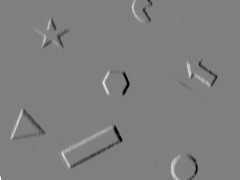
\includegraphics[width =
    \textwidth]{images/variance_contrast.png}
    % \label{subfig:map}
    (b) An optimized frame using variance metric
  \end{minipage}
  \caption{Comparison between two different metrics}
  \label{fig:contrast}
\end{figure}



\subsection{Planar Homography}

\label{sec:planar_homo}
The warp function $\vec{x}'=\mat{W}(\vec{x},t;\bm{\theta})$ does not only
depend on the motion parameters, but also the scene parameters, which
is the unknown depth.  In the case of a planar scene the problems
simplifies, since a plane $\mathbf{P}$ can be parameterized by two
sets of parameters: $\vec{n}\in\mathbb{S}^2$ the unit surface normal
of $\mathbf{P}$ with respect to the current camera frame, and $d$ the
distance from the camera center to $\mathbf{P}$. The warp function
then becomes
\begin{align}
  \vec{X}'=&\mat{R}(t)\vec{X}+\vec{T}(t)\\
  \vec{X}=&\mat{R}(t)^\top\left(\vec{X}'-\vec{T}(t)\right)\\
  \vec{X}=&\mat{R}(t)^\top\left(\mat{I}+\vec{T}(t)\vec{n}^\top/d\right)\vec{X}',  \label{eq:planar_homo_0}
\end{align}
thus
$\vec{x}'\sim\left(\mat{R}(t)^\top\left(\mat{I}+\vec{T}(t)\vec{n}^\top/d\right)\right)^{-1}\vec{x}$.
Here $(\mat{R}(t), \vec{T}(t))\in SE(3)$ denotes the relative pose
between two cameras at which the current event being warped and the
first event within the window happened, and $t$ is the relative
timestamp with respect to the first event. Under a constant velocity
model with linear velocity $\vec{v}\in\mathbb{R}^3$ and angular
velocity $\bm{\omega}\in\mathbb{R}^3$, the translation is given by
\begin{equation}
  \label{eq:translation}
  \vec{T}(t)=\vec{v}t,
\end{equation}
the rotation matrix is given by the \textit{exponential map} exp:
$\mathfrak{so}(3)\rightarrow SO(3)$:
\begin{equation}
  \label{eq:rotation}
  \mat{R}(t)=\mathrm{exp}(\bm{\omega}^\wedge t),
\end{equation}
where $^\wedge$ is the \textit{hat} operator
\begin{equation}
  \label{eq:hat}
  \bm{\omega}^\wedge=
  \begin{bmatrix}
    \omega_1\\\omega_2\\\omega_3
  \end{bmatrix}
  =
  \begin{bmatrix}
    0&-\omega_3&\omega_2\\
    \omega_3&0&-\omega_1\\
    -\omega_2&\omega_1&0
  \end{bmatrix}
  \in\mathfrak{so}(3).
\end{equation}

\section{From Frames to Map}
\label{sec:frame2map}
The contrast maximization procedure in the above section optimizes the
relative pose between successive frames. We show in this section that
the same idea can be applied to perform global pose tracking in planar
scenes. We first explain how the map is defined, and how to track a
known map, then we shown how this map is built by selecting a set of
keyframes.

\subsection{Map}
\label{sec:map}
A map is a plane with three components: the normal direction
$\vec{n}_w$, the distance $d_w$ to the origin, and the texture; the
texture of a map represents all the edges on the plane. \Cref{fig:map}
shows the an example of such map. \Cref{fig:map}(a) also shows the set
of keyframes used to construct the map. We will talk more about
keyframes in \cref{sec:keyframe2map}. The global coordinate is chosen
as the camera coordinate of the first frame.

\begin{figure}
  \begin{minipage}[t]{0.48\textwidth}
    \centering 
\includegraphics[width =
    \textwidth]{images/map_805.jpg}
    % \label{subfig:texture}
    (a) The texture of a map
  \end{minipage}
  \hfill
  \begin{minipage}[t]{0.48\textwidth}
    \centering 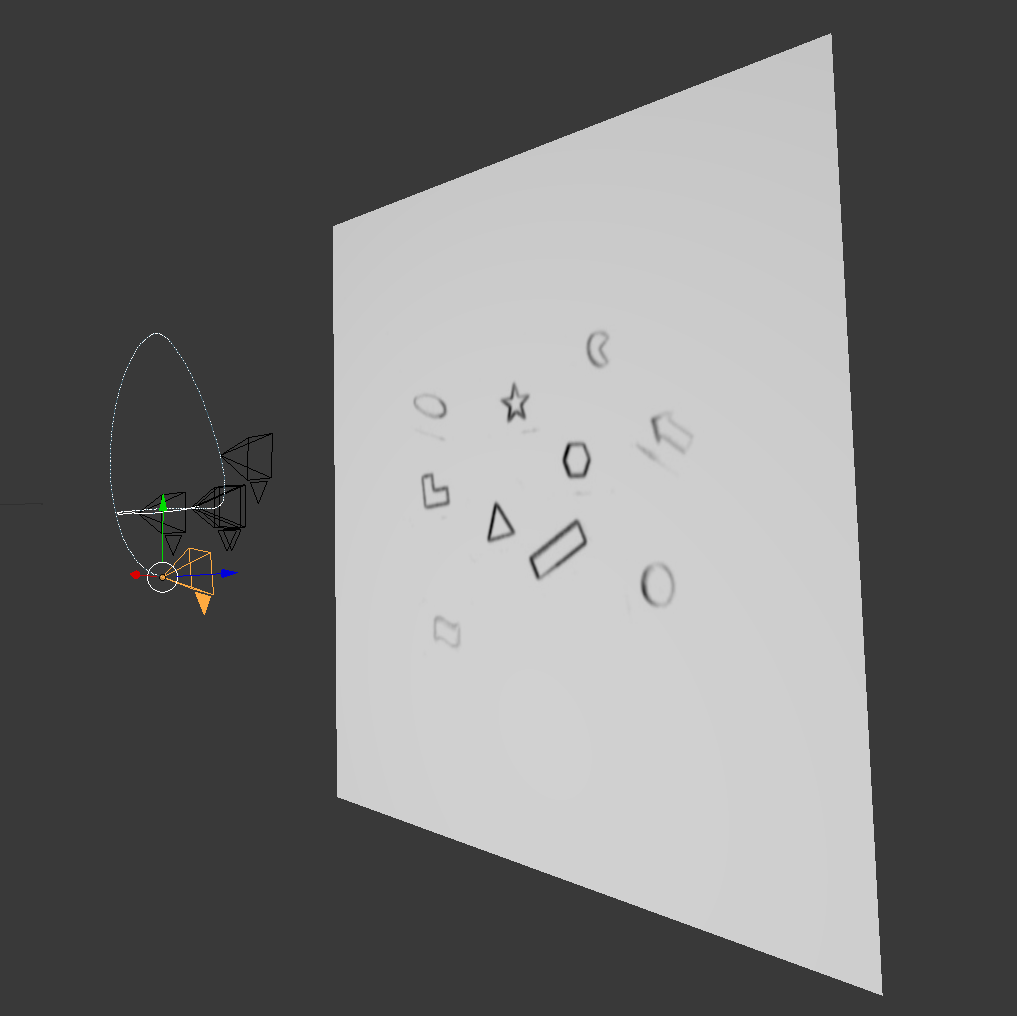
\includegraphics[width = \textwidth]{images/4.png}
    % \label{subfig:map}
    (b) A map in the global frame
  \end{minipage}
  \caption{Map}
  \label{fig:map}
\end{figure}



\subsection{Tracking}
\label{sec:tracking}
Suppose a map is present, then the normal direction $\vec{n}_w$ of the
plane and the distance $d_w$ to the origin are known. Also the pose of
the current frame $(\mat{R}_{wc}, \vec{T}_{wc})\in SE(3)$ is
determined by the motion estimation from the last frame (a quick note
to the terminology we are using: whenever we say the \textit{pose} of
a frame, we always refer to the camera \textit{pose} at which the
first event within the frame happens). The parameters left to be
estimated for each frame is
$\phi=\left(\bm{\omega},\vec{v}\right)\in\mathbb{R}^6$. By
substituting $\vec{n}$ with $\vec{n}_c = \mat{R}_{cw}\vec{n}_w$, and
$d$ with $d_c = d_w+\vec{T}_{wc}\cdot\vec{n}_w$ in
\cref{eq:planar_homo_0}, we get the homography matrix within each
frame as
\begin{equation}
  \label{eq:planar_homo_1}
  \mat{H}_1=\mat{R}^\top\left(\mat{I}+\vec{T}\vec{n}_c^\top/d_c\right)
\end{equation}
and $\vec{x}'_c\sim\mat{H}_1^{-1}x_c$.

A nonlinear optimizing problem naturally suffers from local
optima. Without a good initialization, the motion computed with the
method in \cref{sec:event_warp} could sometimes be a local optimum
delivering an image that appears sharp, despite being wrongly
estimated (see \cref{fig:local_optimum}). In order to make sure that
the estimated motion from the per frame contrast maximization also
conform to the global map. Thus we perform another optimization, where
we project the events of the current frame to the global map. The
parameter set is still $\left(\bm{\omega}^\top,\vec{v}^\top\right)$,
and we use the output from last procedure as an initial guess.

The procedure described in the first paragraph of this section can be
understood as projecting the events on a \textit{blank
  canvas}. Similarly, in the projecting-to-map procedure we project
the events on the \textit{texture} of the map, and measure the
strength of the synthesized image with the same variance function as
in \cref{eq:variance}, thus finding the set of the parameters that
best align the events in the current frame to their correspondences in
the texture.

The projection from an event to the map is
\begin{equation}
  \label{eq:frame2map}
  \vec{x}_w \sim \mat{R}_n\mat{H}_2^{-1}\mat{H}_1^{-1}\vec{x}_c,
\end{equation}
with $\mat{R}_n$ the transformation from the orientation of the global
frame to the orientation of the map, computed by
\begin{align}
  \mat{K}& =(\vec{n}_w\times \vec{z})^\wedge\\
  \mat{R}_n&=\mat{I} +\mat{K} + \mat{K}^2/ (1 +  \vec{n_w}\cdot\vec{z}),  \label{eq:global2map}
\end{align}
where $\vec{z}=(0,0,-1)$ denotes the plane fronto-parallel to the
camera, and
\begin{equation}
  \label{eq:frame2global}
  \mat{H}_2 = \mat{R}_{cw}\left(\mat{I} + \vec{T}_{wc}\vec{n}^\top/d_w\right)
\end{equation}
is the projection from the current frame to the global frame, with
$\mat{R}_{wc}, \mat{T}_{wc}$ being the pose of the current
frame. $\mat{H}_1$ is the planar homography for each frame as in
\cref{eq:planar_homo_1}. But the $\mat{R}(t)$ and $\vec{T}(t)$ might
be different since we are refining these parameters.

After projecting, we obtain an image composed of the map texture and
the events of the current frame. We maximize the contrast of this
image using the cost function defined in \cref{eq:variance}. The
optimized velocity is used for propagating the pose to the next
incoming frame via
\begin{align}
  \label{eq:pose_propagation}
  \vec{T}_{wc_2}&=\mat{R}_{wc_1}\vec{v}\Delta t+ \vec{T}_{wc_1}\\
  \mat{R}_{wc_2}& =\mat{R}_{wc_1}\mathrm{exp}(\bm{\omega}^\wedge \Delta t),
\end{align}
where $c_1$ and $c_2$ denotes the current frame and the next frame,
respectively, and $\Delta t$ is the temporal size of the current
frame.

\begin{figure}
  \begin{minipage}[t]{0.48\textwidth}
    \centering 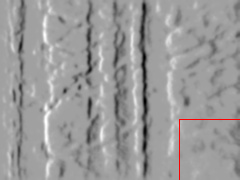
\includegraphics[width =
    \textwidth]{images/slider_estimation.png}
    \label{subfig:estimation}
    (a) Estimation
  \end{minipage}
  \hfill
  \begin{minipage}[t]{0.48\textwidth}
    \centering 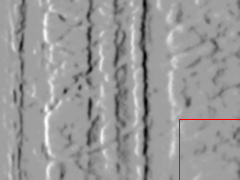
\includegraphics[width =
    \textwidth]{images/slider_groundtruth.png}
    \label{subfig:groundtruth}
    (b) Groundtruth
  \end{minipage}
  \hfill

  \begin{minipage}[t]{\textwidth}
    \centering 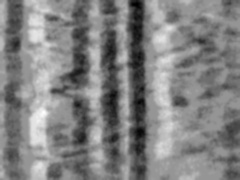
\includegraphics[width =
    0.48\textwidth]{images/slider_zero_motion.jpg}
    \label{subfig:estimation}
    \\(c) Without motion compensation
  \end{minipage}
  \hfill

  \caption{An example of local optima. This is the dataset
    \textit{slider\_hdr\_close} with a window size of 50000
    events. (a) shows the optimized image with \textit{linear
      velocity} $( 0.231, 0.109, 0.256)$, \textit{angular velocity}
    $(0.405, -0.130, -0.278)$ and \textit{plane normal}
    $(-0.579, 0.282, -0.765)$. (b) shows the result using groundtruth
    parameters with \textit{linear velocity} $(0.163, 0, 0)$,
    \textit{angular velocity} $(0, 0, 0)$ and \textit{plane normal}
    $(0, 0, -1)$. Both images appear mostly identical, though at the
    lower right corner, for example, one can still recognize the
    difference. Also both images look much sharper than the image
    without motion compensation in (c). It is worth mentioning that
    the contrast of the estimation is actually slightly larger than
    that of the groundtruth}
  \label{fig:local_optimum}
\end{figure}

\subsection{Mapping}
\label{sec:keyframe2map}

After having collected the first $N$ events, we start the mapping
process. For the first frame we estimate the full parameter set
$\phi=\left(\bm{\omega}^\top,\vec{v}^\top/d_w,\varphi,\psi\right)^\top\in\mathbb{R}^8$,
where $\left(\varphi, \psi\right)$ parametrize the unit vector of the
plane normal, and $\vec{v}^\top/d_w$ account for the scale ambiguity
problem introduced in linear velocity estimation from monocular
camera. We can for example determine the scale of the scene by setting
$d_w$ to $1m$, then scales of the consecutive frames are also
determined by $d_c = d_w+\vec{T}_{wc}\cdot\vec{n}_w$.

From the optimized first frame we initialize the map, by projecting
the frame to the planar scene via a rotation $\mat{R}_n$ as in
\cref{eq:global2map} \textcolor{red}{(you might have implemented this
  part wrong)}. Then we can track the next frames with this map using
the method described in \cref{sec:tracking}.

As the camera moves, there might be new information available in the
scene, so that the map needs to be expanded. After optimization for
each single frame, we also measure the \textit{per-pixel-overlap}
between the frame and the map,S that is, how many percent pixels in the
frame can be explained by the map. The overlap might be small, when
the camera is just exploring a new area so that only part of the frame
and the map is overlapping; another possibility is that the map is not
accurate enough to explain the current frame, which often happens when
only one frame is used until now to construct the map. When the
overlap reaches a certain threshold (0.8 for example), we try to
insert a new \textit{keyframe}.

When the system decides that a new keyframe is needed, we collect all
the keyframes until now, plus the current frame, which is a keyframe
candidate, and optimize the poses and velocities of these frames, as
well as the map together. Suppose there are $k$ frames (including the
keyframe candidate), the to be optimized parameter set is
\begin{equation*}
  \phi=\left(\mat{R}_{(1\sim k)},\vec{T}_{(1\sim
      k)},\bm{\omega}_{(0\sim k)},\vec{v}_{(0\sim
      k)}/d_w,\varphi,\psi\right)\in\mathbb{R}^{12k-4}.
\end{equation*}
Here $1\sim k$ means from frame $1$ to frame $k$, and we skip the pose
optimization of frame $0$, which is the first frame, since it defines
the global coordinate. We project all the events of these $k$ frames
to the plane parametrize by $(\varphi,\psi)$ with \cref{eq:frame2map},
and again optimize the contrast of the synthesized image the obtain
the optimal parameter set.

Note that in the mapping process we drop the polarity of the event,
since different keyframes might include events from the same visual
stimuli but triggered when moving in different directions, when summed
together the polarities might cancel each other out. For the same
reason, we also don't use the polarity when matching a frame to the
map.

After this step, we also measure the \textit{per-pixel-overlap}
between the keyframe candidate and the image synthesized by the other
keyframes, with the newly optimized parameter set. If this is a good
match \textcolor{red}{(define a good match)}, we continue the
tracking. Otherwise, we consider the pose estimation of the current
frame to be already off. In this case we preserve the former map, and
use this map to start the \textit{relocalization} procedure.

\subsection{Relocalization}
\label{sec:relocalization}

\section{Experiments}
\label{sec:experiments}
The algorithm is tested on four planar datasets provided by the
\textit{Robotics and Perception Group} at UZH
\citep{mueggler2017event}, which includes \textit{poster\_6dof,
  poster\_translation, shapes\_6dof, shapes\_translation}. The
\textit{shapes} dataset contains several simple shapes on the wall,
whereas the \textit{poster} contains richer rock texture. A planar
assumption is redundant for the rotation datasets and thus the results
are not listed for comparison here.

We define the camera axes as in \cref{fig:axes}. The camera coordinate
frame of the first synthesized frame is set as the global coordinate
frame. The x, y and z axes are also pitch yaw, roll axes,
respectively.

\begin{figure}
  \begin{minipage}[t]{0.48\textwidth}
    \centering 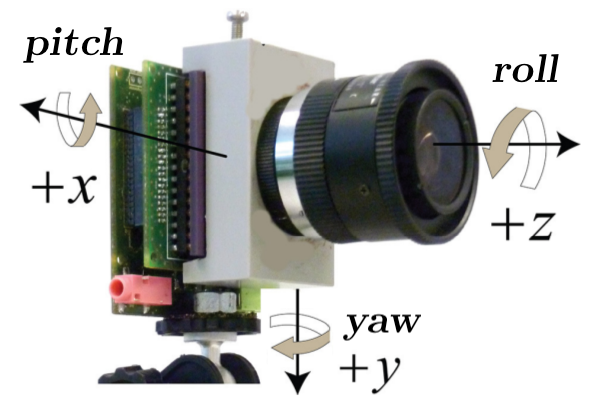
\includegraphics[width = \textwidth]{images/axes.png}
    (a)
  \end{minipage}
  \hfill
  \begin{minipage}[t]{0.48\textwidth}
    \centering 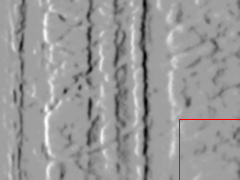
\includegraphics[width =
    \textwidth]{images/slider_groundtruth.png} (b)
  \end{minipage}
  \hfill
  \caption{Axes definition}
  \label{fig:axes}
\end{figure}
\Cref{fig:shapes_6dof_pose} shows the comparison of the results of the
proposed method against ground truth on the whole
\textit{shapes\_6dof} sequence. We observe that the orientation and
translation estimation along z axis is the most accurate among all the
axes; when zoomed in (\cref{fig:shapes_6dof_pose_zoomed}), it is clear
to see that the roll estimation is almost indistinguishable from the
ground truth. We split the quantitative error estimation for
orientation along 3 axes (\cref{tab:err_est}), in order to show that
this holds true for all the datasets we tested on. In these datasets,
the global z axis is close to the plane normal; we believe that the
events generated by a motion along the plane normal direction is more
obvious, and also harder to be explained by a combination of other
motions, and are thus more reliable.

We also observe in \cref{fig:shapes_6dof_pose} that in the latter half
of the sequence there are larger fluctuations. There are multiple
reasons for that:
\begin{enumerate}
\item The window size is not suitable

  The window size is manually chosen for each dataset. A range of
  $2000 - 5000$ usually works good for the \textit{shapes} datasets,
  since the scene consists of simple regular
  shapes. \Cref{fig:window_size}(a) shows what the camera frustum
  normally contains. However, in the rapid movement phase, the camera
  very often moved to a position where other scenes which don't belong
  to \textit{shapes} also becoms visible. \Cref{fig:window_size}(b)
  shows the scene of \textit{shapes\_6dof} at around 47.8 seconds. At
  this moment the poster on the wall is also visible, which actually
  belongs to the \textit{poster} sequences. The poster has much more
  complex textures, when performing pose estimation on the
  \textit{poster} sequences, we normally choose a window size of
  $30000-50000$. Apparently, a window size of 4000 is no longer enough
  in this case, which causes the motion estimation in this period
  being inaccurate.
  \begin{figure}
    \begin{minipage}[t]{0.48\textwidth}
      \centering 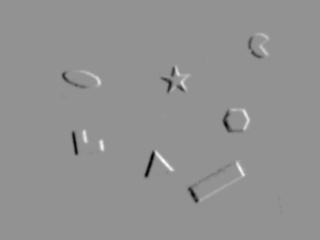
\includegraphics[width =
      \textwidth]{images/window_size_good.jpg} (a)
    \end{minipage}
    \hfill
    \begin{minipage}[t]{0.48\textwidth}
      \centering 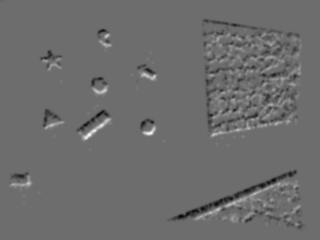
\includegraphics[width =
      \textwidth]{images/window_size_bad.png} (b)
    \end{minipage}
    \hfill
    \caption{A window size of $4000$ for a specific dataset
      \textit{shapes\_6dof} but different scene complexity}
    \label{fig:window_size}
  \end{figure}
\item There are few textures available

  A very representative example is that when tracking the dataset
  \textit{shapes\_translation}, we always get lost at around $23
  sec$. Investigating the scene around this time instance
  (\cref{fig:shapes_tr_lost}(a)), we found that very few or even no
  texture is available. It's also not possible to perform a reliable
  pose estimate during this period. For the \textit{per-frame}
  velocity estimation proposed in
  \citep{gallego2017accurate,gallego2018unifying}, where each frame is
  uncorrelated \textcolor{red}{?}, this is usually not a serious
  problem, since when the textures becomes available again, the
  optimization pipeline is still able to continue, it just might be
  harder to start from a bad initialization. However, for the pose
  estimation where a cumulative result is needed, a few bad estimated
  frames might destroy the whole following sequence.

  The \textit{bundle adjustment} and \textit{relocalization} parts of
  the pipeline is designed to deal with such situations. However, a
  bad initial guess of the pose $(\mat{R},\vec{T})$ is generally
  harder to start with than a bad initial guess of velocities
  $(\bm{\omega},\vec{v})$. When the pose estimation from last frame is
  already too off, after optimization there might still be little
  overlap between the current frame and the pose. This is when the
  \textit{bundle adjustment} tries to insert a keyframe and track from
  the new keyframe. The current implementation doesn't reinitialize
  the map after the tracking is lost. The advantage is that there is
  still chance to come back to the original map after tracking a wrong
  ``local map'' (\cref{fig:shapes_tr_lost}(b)); the disadvantage is
  that the global map will most likely be polluted by the ``local
  map'' (\cref{fig:shapes_tr_lost}(c))
  \begin{figure}
    \begin{minipage}[t]{0.48\textwidth}
      \centering 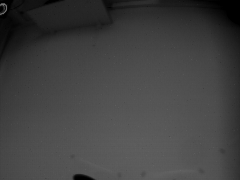
\includegraphics[width =
      \textwidth]{images/frame_00000520.png} (a) There is little
      texture visible
    \end{minipage}
    \hfill
    \begin{minipage}[t]{0.48\textwidth}
      \centering 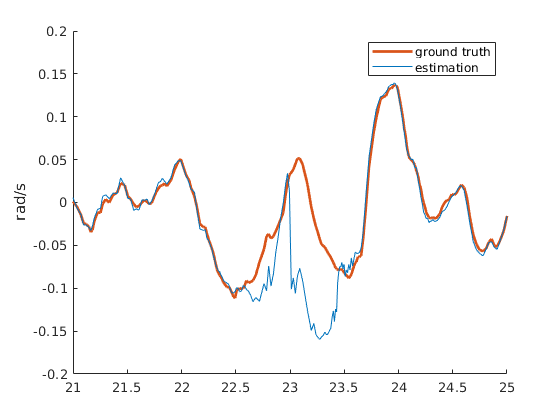
\includegraphics[width =
      \textwidth]{images/shapes_tr_lost.png} (b) Relocalized after get
      lost (roll component)
    \end{minipage}

   \begin{minipage}[t]{0.48\textwidth}
     \centering 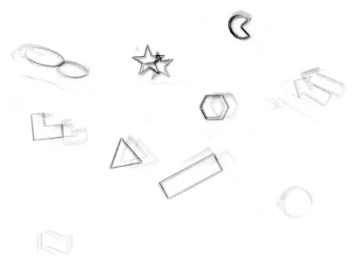
\includegraphics[width =
     \textwidth]{images/map_956.jpg} (c) Polluted map after tracking
     is lost
   \end{minipage} \caption{When tracking the dataset
     \textit{shapes\_translation}, we always get lost at around
     $23 sec$, but there is still chance to relocalize}
   \label{fig:shapes_tr_lost}
 \end{figure}

\end{enumerate}

\begin{figure}
  \begin{minipage}[t]{\textwidth}
    \centering 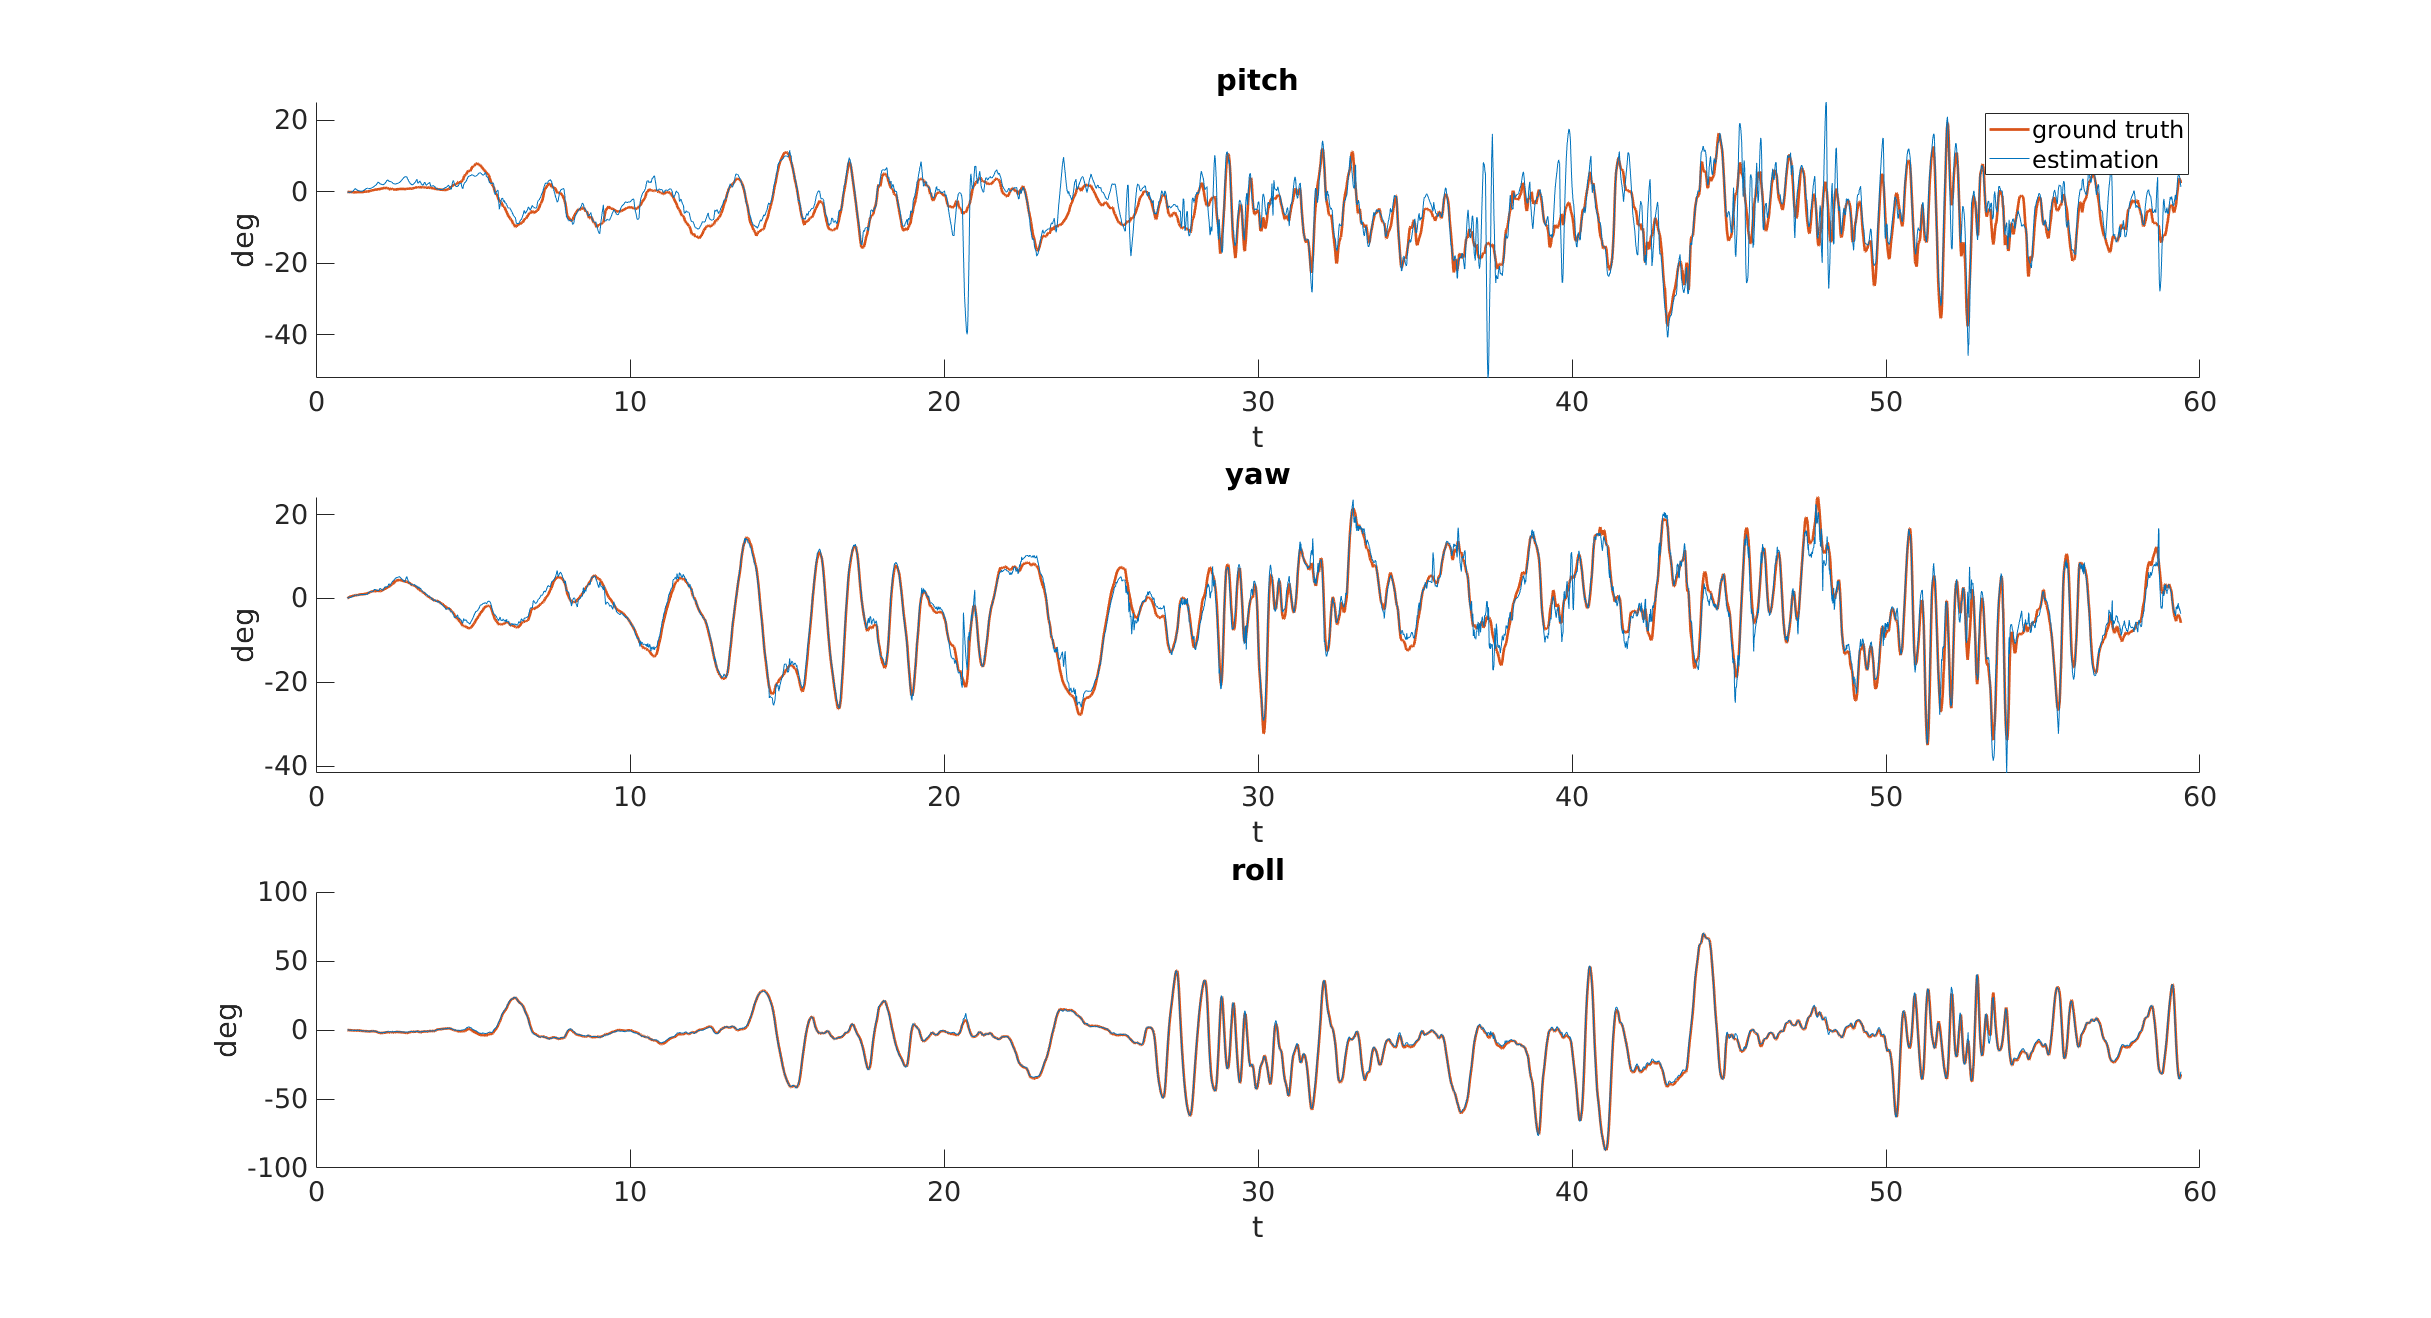
\includegraphics[trim={5cm 0cm 5cm 0cm},clip,width =
    \textwidth]{images/shapes_6dof_rotation.png} (a) Orientation
  \end{minipage}
  \hfill
  \begin{minipage}[t]{\textwidth}
    \centering 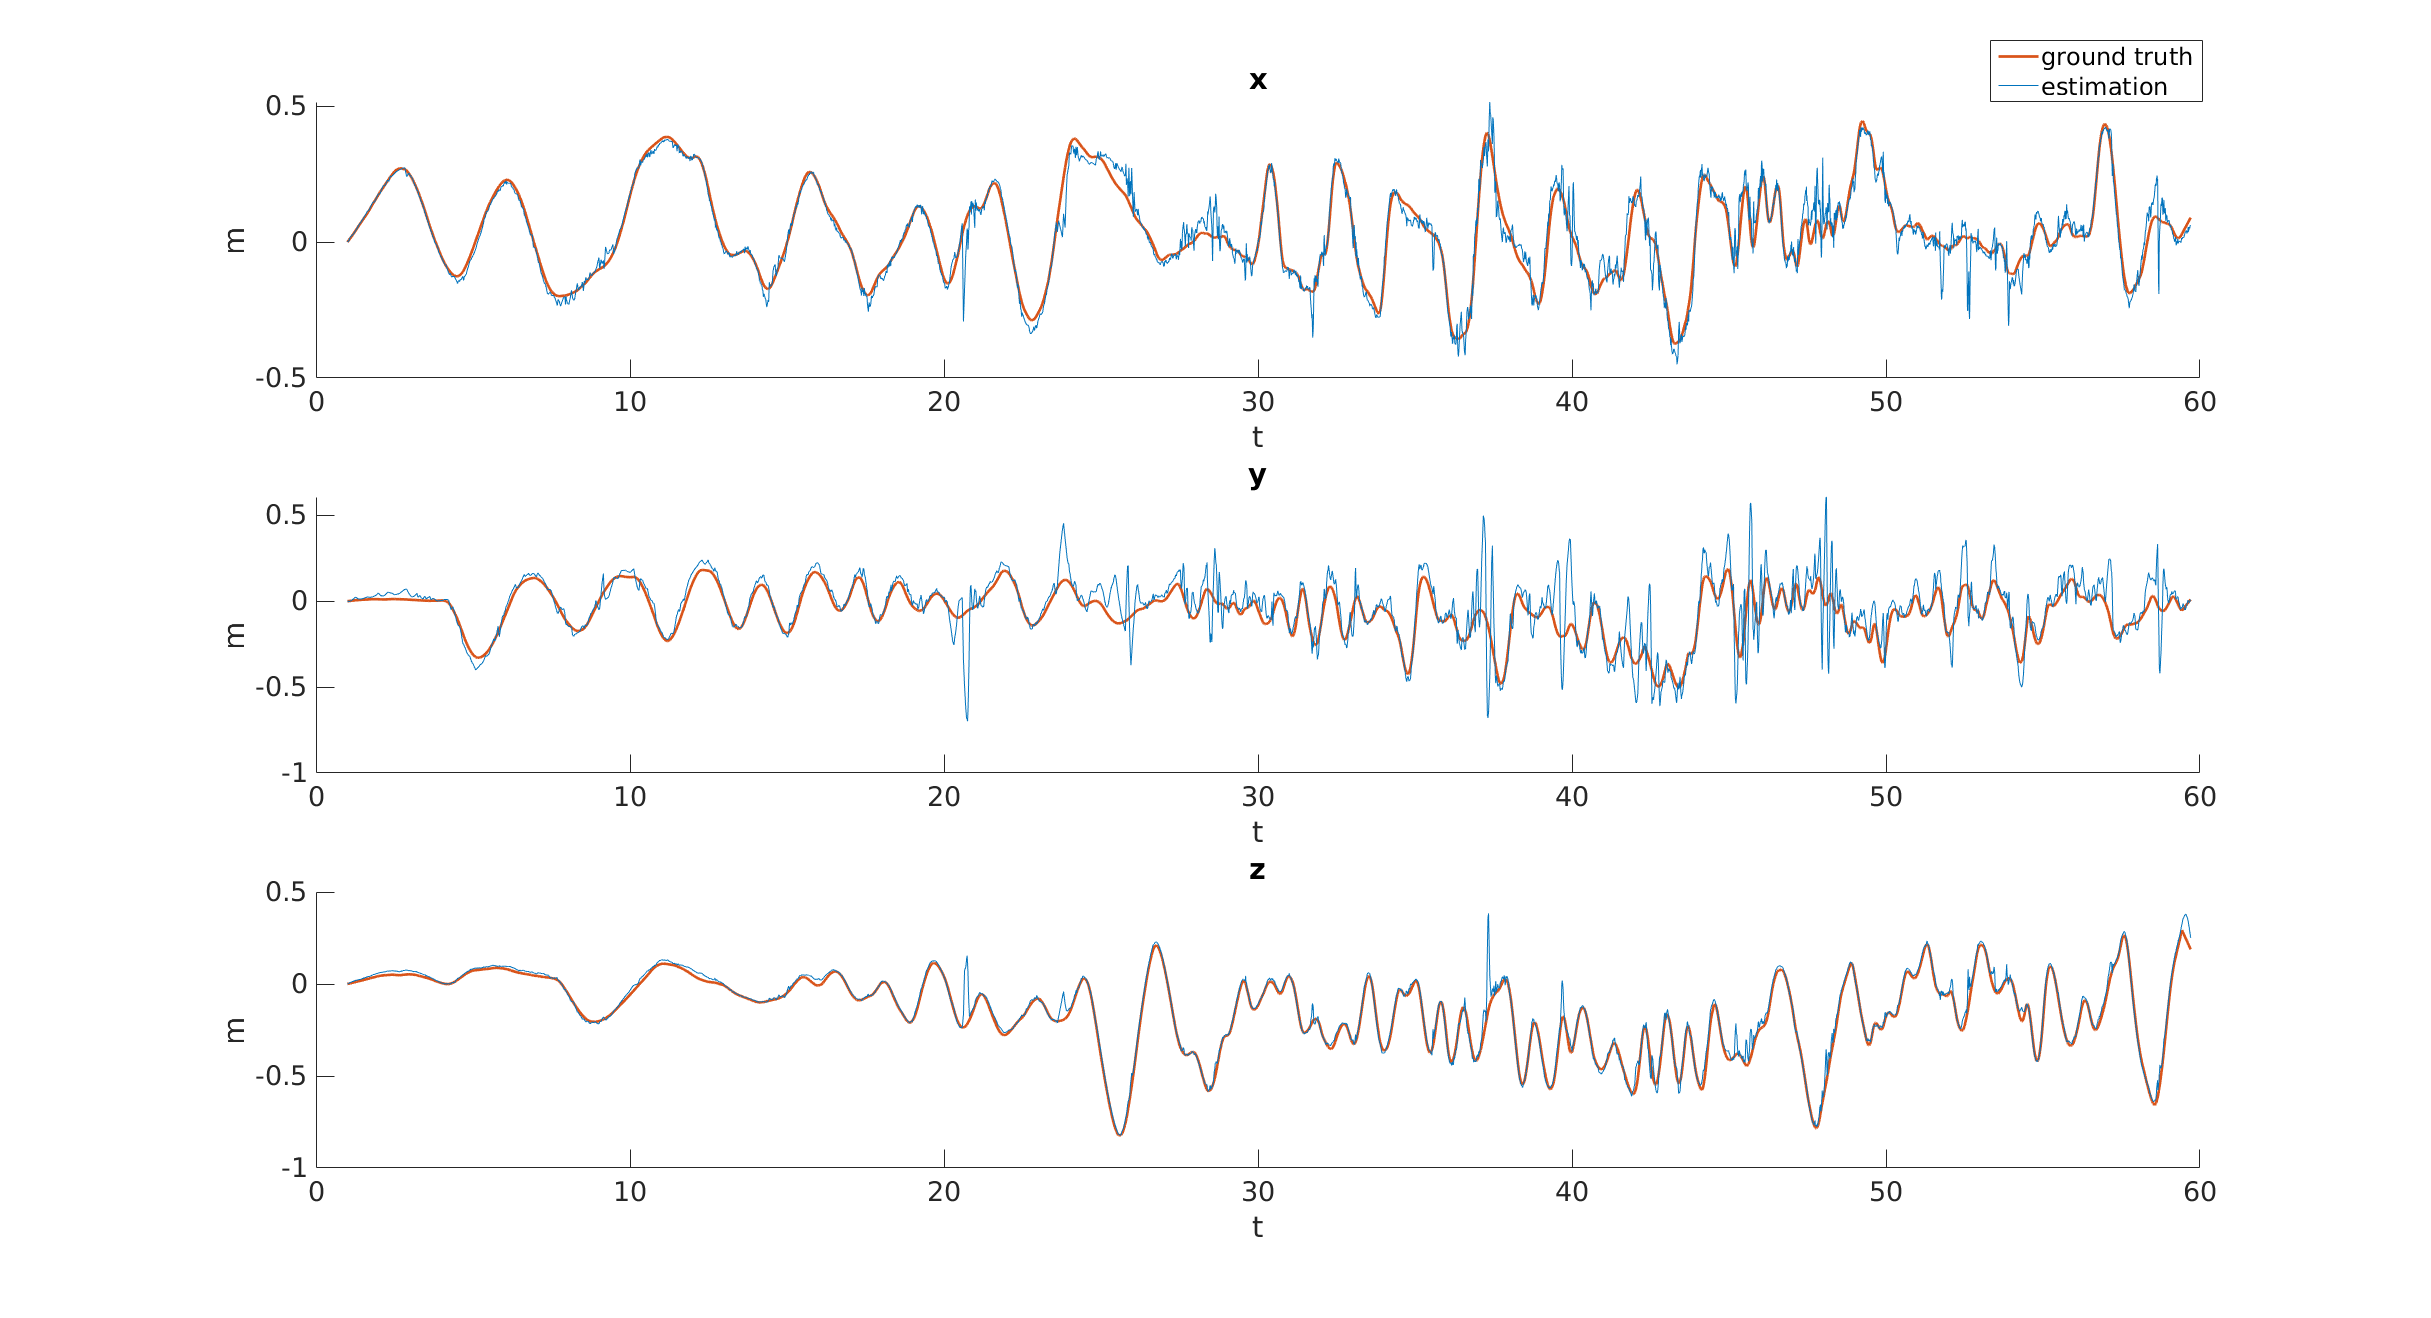
\includegraphics[trim={5cm 0cm 5cm 0cm},clip,width =
    \textwidth]{images/shapes_6dof_translation.png} (b) Translation
  \end{minipage}
  \hfill
  \caption{\textit{shapes\_6dof} sequence. Comparison of the estimated
    pose (blue line) against ground truth (red line).}
  \label{fig:shapes_6dof_pose}
\end{figure}

\begin{figure}
  \begin{minipage}[t]{0.48\textwidth}
    \centering 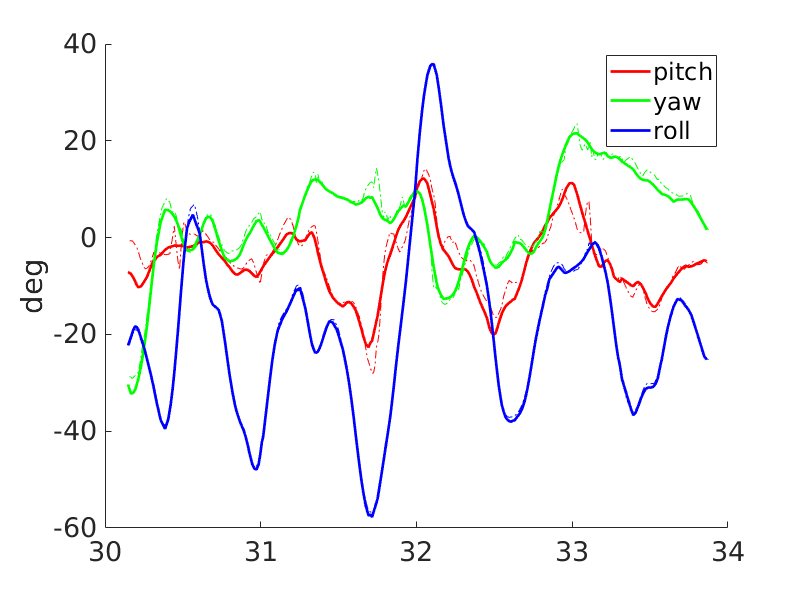
\includegraphics[width =
    \textwidth]{images/shapes_6dof_rotation_33.png} (a) Orientation
  \end{minipage}
  \hfill
  \begin{minipage}[t]{0.48\textwidth}
    \centering 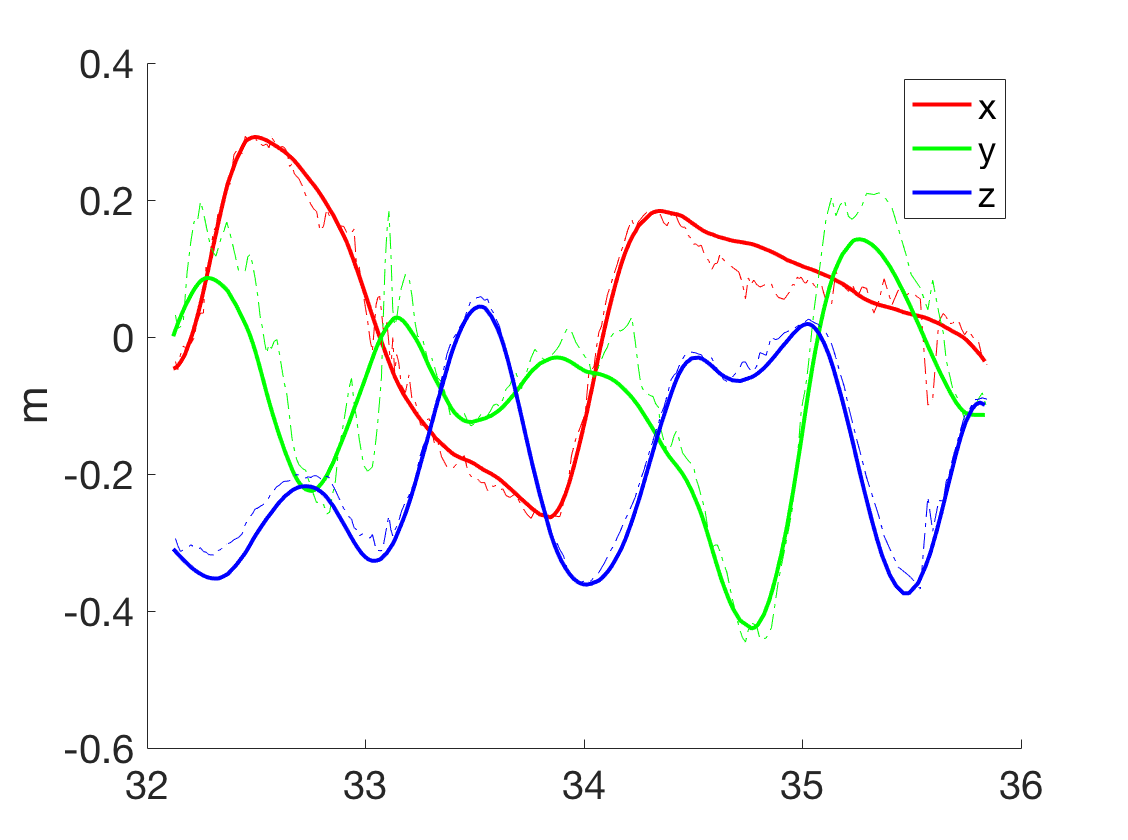
\includegraphics[width =
    \textwidth]{images/shapes_6dof_translation_33.png} (b) Translation
  \end{minipage}
  \hfill
  \caption{\textit{shapes\_6dof} sequence. Comparison of the estimated
    pose (dashed line) against ground truth (full line) within
    segments of 8 seconds duration.}
  \label{fig:shapes_6dof_pose_zoomed}
\end{figure}
A quantitative error estimation is included in \cref{tab:err_est}. The
window sizes for \textit{shapes} and \textit{poster} sequences are
4000 and 30000, respectively. Also, we used the \textit{Nelder-Mead
  Simplex} algorithm provided by \textit{gsl} to perform the
optimization on \textit{shapes} sequences, and the
\textit{Fletcher-Reeves conjugate gradient} algorithm to perform
optimization on the \textit{poster} dataset. Both methods work. The
analytic differentiation is faster and more stable. However, when the
initial guess is further from the ground truth, the numeric
differentiation seems to work better than the analytic
differentiation, since the jacobians used for analytic differentiation
are strictly local (see appendix). whereas a properly chosen step size for numeric
differentiation
\begin{itemize}
\item median\\
  \item scene depth no drift\\
\end{itemize}

\begin{table}[h]
  \label{tab:err_est}
  \begin{center}
    \begin{tabular}{lcccccl}
      \hline
      \multirow{3}{*}{Dataset}&\multicolumn{3}{c}{Median Orientation}&\multirowcell{3}{Median Translation \\ Error/m}&\multirowcell{3}{Traveled\\Distance}&\multirow{3}{*}{Note}\\
                              &\multicolumn{3}{c}{Error/deg}& &\\
      \cline{2-4}
                              & pitch&  yaw & roll &       &       &                  \\
      \hline
      shapes\_6dof        & 1.89 & 1.01 & 0.85 & 0.047 & 46.89 & Tracked all 60s  \\
      shapes\_translation & 0.85 & 0.45 & 0.27 & 0.019 & 14.08 & Lost after 25.0s \\
      poster\_6dof        & 1.14 & 1.22 & 0.63 & 0.054 & 12.50 & Lost after 22.8s \\
      poster\_translation & 0.55 & 0.57 & 0.25 & 0.022 & 11.14 & Lost after 26.0s \\
      \hline
    \end{tabular}
  \end{center}
  \caption{Quantitative evaluation on planar sequences}
\end{table}


% \begin{table}[h]
%   \label{tab:err_est}
%   \begin{center}
%     \begin{tabular}{lcccccccl}
%       \hline
%       &\multicolumn{3}{c}{Median Orientation}& \multicolumn{3}{c}{Median Translation}&Travelled Distance&Note \\
%       Dataset&\multicolumn{3}{c}{Error/deg}& \multicolumn{3}{c}{Error/m}&\\
%       \cline{2-9}
%       & pitch & yaw&roll&x&y&z&& \\
%       \hline
%       shapes\_6dof        & 1.47 & 2.94 &1.39 &0.019&0.036&0.014&46.89&med 0.0474     \\
%       shapes\_translation & 1.02 & 1.85 &0.31 &0.010 &0.021 &0.012&11.46&med 0.0292 \\
%       poster\_6dof& stuffed     & 92.50  &&0.027&0.018&0.035&12.5&med 0.054    lost after 22.8s    \\
%       poster\_translation& 0.55     & 0.57   &0.25&0.009&0.010&0.014&11.14&med 0.0221  lost after 26.03s \\
%       \hline
%     \end{tabular}
%   \end{center}
%   \caption{Quantitative evaluation on planar sequences}
% \end{table}


Despite of the rapid movements, in the above datasets the camera
actually only moves in a relative small region in front of the
textured plane, as depicted in \cref{fig:shapes_6dof_path}. However,
this method also applies when camera travels a longer distance with
respect to the scene depth, as shown in
\cref{fig:slider_hdr_far_map}. Also, although this method is designed
for planar scenes, in a complex scene with rotation only movement,
where no scene parameters are needed, this method can still be applied
to build a global map, delivering a result similar to \textit{image
  stitching}. \Cref{fig:boxes_rotation_map} is such an example.
\begin{figure}
  \centering
  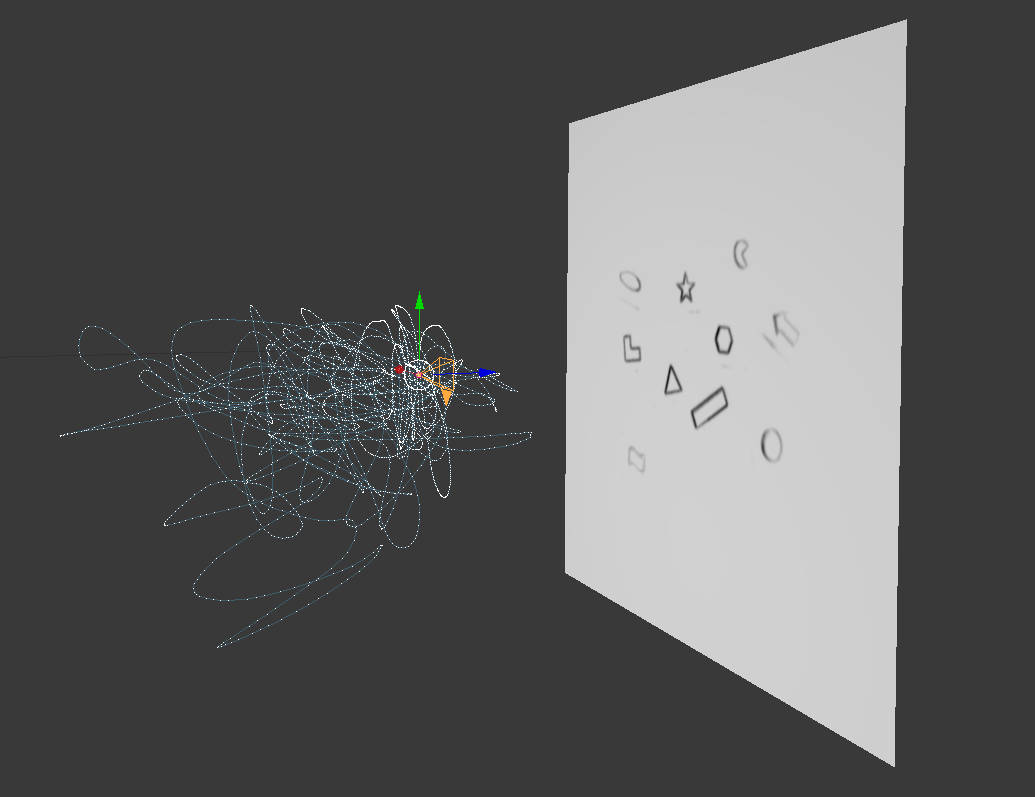
\includegraphics[width=\textwidth]{images/shapes_6dof_path.png}
  \caption{The motion path of the dataset
    \textit{shapes\_6dof}. Despite a trajectory length of about $50m$,
    in the whole $60s$ the camera actually stays in a relative small
    region compared to the scene depth, and there is no observable
    increase of drift using the method in this
    work. \textcolor{red}{ref to error estimation}}
  \label{fig:shapes_6dof_path}
\end{figure}
\begin{figure}
  \centering
  
\includegraphics[width=\textwidth]{images/slider_hdr_far_map_36.jpg}
  \caption{The dataset \textit{slider\_hdr\_far}, with a scene depth
    of $0.584 m$, and a camera movement in the positive $x$ direction
    only. Note that this is a much wider map than what we have seen
    before. The figure shows the result at $4.8 sec$ within the whole
    range of $6.3 sec$; afterwards the algorithm is lost in the
    forest, where almost all the textures are vertical, causing severe
    local optima problem. If we constrain the motion estimation to
    translation only, it delivers a much better result.}

  \label{fig:slider_hdr_far_map}
\end{figure}
\begin{figure}
  \centering
  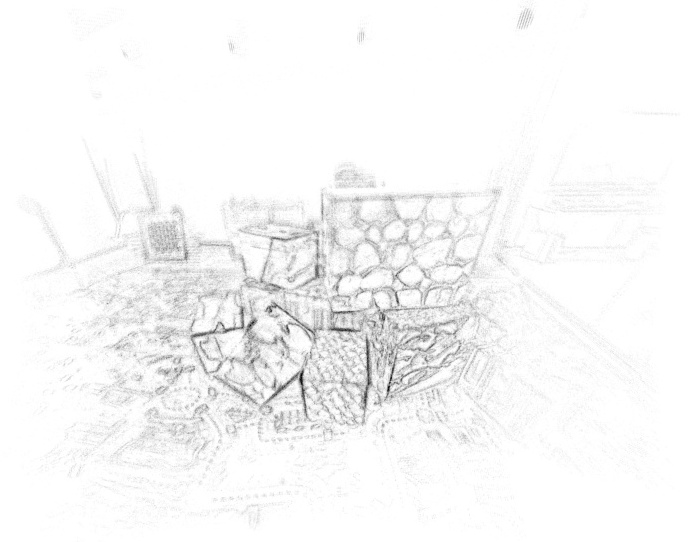
\includegraphics[width=\textwidth]{images/boxes_rotation_map.jpg}
  \caption{The dataset \textit{boxes\_rotation}. The motion in this
    dataset is rotation-dominated}
  \label{fig:boxes_rotation_map}
\end{figure}




\chapter{A Discussion to 6DoF Motion Estimation in General 3D Scenes}
\label{chap:general_scene}



\subsection{note}
\label{sec:note}

tried initialize with multiple frames, didn't work very
well. similarly sliding window didn't work; too many events didn't
work

\chapter{Discussion}
\label{chap:discussion}


\section{Erstellen einer Tabelle}\label{sec:tabellen}

Ein Beispiel einer Tabelle:
\begin{table}[h]
  \begin{center}
    \caption{Daten der Fahrzyklen ECE, EUDC, NEFZ.}\vspace{1ex}
    \label{tab:tabnefz}
    \begin{tabular}{ll|ccc}
      \hline
      Kennzahl & Einheit & ECE & EUDC & NEFZ \\ \hline \hline
      Dauer & s & 780 & 400 & 1180 \\
      Distanz & km & 4.052 & 6.955 & 11.007 \\
      Durchschnittsgeschwindigkeit & km/h & 18.7 &  62.6 & 33.6 \\
      Leerlaufanteil & \% & 36 & 10 & 27 \\
      \hline
    \end{tabular}
  \end{center}
\end{table}

Die Tabelle wurde erzeugt mit:
\begin{verbatim}
\begin{table}[h]
  \begin{center}
    \caption{Daten der Fahrzyklen ECE, EUDC, NEFZ.}\vspace{1ex}
    \label{tab:tabnefz}
    \begin{tabular}{ll|ccc}
      \hline
      Kennzahl & Einheit & ECE & EUDC & NEFZ \\ \hline \hline
      Dauer & s & 780 & 400 & 1180 \\
      Distanz & km & 4.052 & 6.955 & 11.007 \\
      Durchschnittsgeschwindigkeit & km/h & 18.7 &  62.6 & 33.6 \\
      Leerlaufanteil & \% & 36 & 10 & 27 \\
      \hline
    \end{tabular}
  \end{center}
\end{table}
\end{verbatim}

\section{Weitere nützliche Befehle}\label{sec:div}

Hervorhebungen im Text sehen so aus: \emph{hervorgehoben}. Erzeugt
werden sie mit dem \texttt{\textbackslash epmh\{.\}} Befehl.

Einheiten werden mit den Befehlen \texttt{\textbackslash unit[1]\{m\}}
(z.B.~\unit[1]{m}) und \texttt{\textbackslash unitfrac[1]\{m\}\{s\}}
(z.B.~\unitfrac[1]{m}{s}) gesetzt.
 \cleardoublepage
% \input{} \cleardoublepage \input{} \cleardoublepage ...
%

%%%%%%%%%%%%%%%%%%%%%%%%%%%%%%%%%%%%%%%%%%%%%%%%%%%%%%%%%%%%%%%%%%%%%%%%%%%%%%%
% Bibliography
%%%%%%%%%%%%%%%%%%%%%%%%%%%%%%%%%%%%%%%%%%%%%%%%%%%%%%%%%%%%%%%%%%%%%%%%%%%%%%%
\bibliographystyle{bibliography/IEEEtranN}
\bibliography{bibliography/references}
\addcontentsline{toc}{chapter}{Bibliography} \cleardoublepage

%%%%%%%%%%%%%%%%%%%%%%%%%%%%%%%%%%%%%%%%%%%%%%%%%%%%%%%%%%%%%%%%%%%%%%%%%%%%%%%
% Appendix
%%%%%%%%%%%%%%%%%%%%%%%%%%%%%%%%%%%%%%%%%%%%%%%%%%%%%%%%%%%%%%%%%%%%%%%%%%%%%%%
\appendix
\chapter{Derivative of the Contrast Metric}\label{sec:jacobian}
Since we use bilinear voting to evaluate the \textit{dirac delta}, the
derivatives of the cost function \cref{eq:variance} can be
analytically computed as
\begin{align}
  \intertext{Let}
  \rho\left(\vec{x};\bm{\theta}\right)&=\mathcal{I}\left(\vec{x};\bm{\theta}\right)-\mu\left(\mathcal{I}\left(\vec{x};\bm{\theta}\right)\right)\\
  \intertext{Then}
  \frac{\partial}{\partial\bm{\theta}}\mathrm{Var}\left(\mathcal{I}\left(\vec{x};\bm{\theta}\right)\right)&=\frac{2}{\mid\Omega\mid}\int_{\Omega}\rho\left(\vec{x};\bm{\theta}\right)\frac{\partial\rho\left(\vec{x};\bm{\theta}\right)}{\partial{\bm{\theta}}}d\vec{x}    \label{eq:dVdw}
\end{align}
The derivatives of the warped image are
\begin{equation}
  \label{eq:dIdw}
  \frac{\partial\mathcal{I}\left(\vec{x};\bm{\theta}\right)}{\partial{\bm{\theta}}}=-\sum_{k=1}^N\pm_k\nabla\delta\left(\vec{x}-\vec{x}'_k\left(\bm{\theta}\right)\right)\frac{\partial\vec{x}'_k\left(\bm{\theta}\right)}{\partial\bm{\theta}},
\end{equation}
In the case of planar homography the events warping is computed as
\begin{align}
  \bm{\theta}&=\left(\bm{\omega}^\top,\vec{v}^\top,\varphi,\psi\right)^\top\in\mathbb{R}^8\\
  \vec{x}'_k\left(\bm{\theta}\right)&=
                                      \begin{bmatrix}
                                        x'_{im}&y'_{im}&1
                                      \end{bmatrix}^\top=
                                                         \begin{bmatrix}
                                                           x'/z'&y'/z'&1
                                                         \end{bmatrix}^\top\\
  \bar{\vec{x}}'_k\left(\bm{\theta}\right)&=
                                            \begin{bmatrix}
                                              x'&y'&z'
                                            \end{bmatrix}^\top\nonumber\\&=
  \mat{P}\left(\mat{R}(t)^\top\left(\mat{I}+\vec{T}(t)\vec{n}^\top/d\right)\right)^{-1}\vec{x}_k\nonumber\\
             &=
               \mat{P}\left(\mat{I}+\vec{v}t\vec{n}^\top\right)^{-1}\mat{R}(t)\vec{x}_k, \label{eq:x_x}
               % &=
               % \mat{P}\left(\mat{I}-\frac{\vec{v}t\vec{n}^\top}{\vec{n}^\top\vec{v}t+1}\right)\mathrm{exp}(\bm{\omega}^\wedge
               % t)\vec{x}_k,
\end{align}
where $\mat{P}$ is the projection matrix from the camera frame to the
world frame or the map, which does not have to correspond with the
camera matrix provided by the dataset. Also, for simplicity of
notation we assume $d = 1$, and denote
$\mat{P}\left(\mat{I}+\vec{v}t\vec{n}^\top\right)^{-1}$ as
$\mat{P_v}$. Since $t$ usually spans a small temporal window, we can
simplify the derivative with respect to angular velocity as
\begin{align}
  \mat{R}(t)& =\mathrm{exp}(\bm{\omega}^\wedge t)\approx\mat{I}+\bm{\omega}^\wedge t\\
  \frac{\partial\bar{\vec{x}}'_k}{\partial\bm{\omega}}&=-\mat{P_v}t\vec{x}_k^\wedge.  \label{eq:dxdo}
\end{align}
The above equation makes use of the equivalence
$\bm{\omega}\times\vec{x}_k=-\vec{x}_k\times\bm{\omega}$.

The derivative with respect to the linear velocity is
\begin{align}
  \frac{\partial\bar{\vec{x}}'_k}{\partial\vec{v}}&=-\frac{t\vec{n}^\top\mat{R}(t)\vec{x}_k}{\vec{n}^\top\vec{v}t+1}\mat{P_v} \label{eq:dxdv}\\
  eu
\end{align}
Similarly we have
\begin{align}
  \frac{\partial\bar{\vec{x}}'_k}{\partial\vec{n}}&=-\frac{t\vec{v}^\top\mat{R}(t)\vec{x}_k}{\vec{n}^\top\vec{v}t+1}\mat{P_v} \\
  \intertext{and}
  \frac{\partial\bar{\vec{x}}'_k}{\partial(\varphi;\psi)}&= \frac{\partial\bar{\vec{x}}'_k}{\partial\vec{n}}\frac{\partial\vec{n}}{\partial(\varphi;\psi)},\\
  \intertext{with}
  \frac{\partial\vec{n}}{\partial(\varphi;\psi)}&=
                                                  \begin{bmatrix}
                                                    -\sin\varphi\sin\psi&\cos\varphi\cos\psi\\
                                                    \cos\varphi\sin\psi&\sin\varphi\cos\psi\\
                                                    0&-\sin\psi
                                                  \end{bmatrix}
                                                       \label{eq:dvdn}
\end{align}
With the above quantities
\begin{equation*}
  \label{eq:dx_dtheta}
  \frac{\partial\bar{\vec{x}}'_k}{\partial\bm{\theta}}=
  \begin{bmatrix}
    \frac{\partial\bar{\vec{x}}'_k}{\partial\bm{\omega}}&
    \frac{\partial\bar{\vec{x}}'_k}{\partial\vec{v}}&
    \frac{\partial\bar{\vec{x}}'_k}{\partial\varphi}&\frac{\partial\bar{\vec{x}}'_k}{\partial\psi}
  \end{bmatrix}\in\mathbb{R}^{3\times8}
\end{equation*}
we can compute the gradient
$\frac{\partial\vec{x}'_k}{\partial\bm{\theta}}$ as
\begin{equation}
  \label{eq:dxdtheta}
  \frac{\partial\vec{x}'_k}{\partial\bm{\theta}}=\frac{\partial\bar{\vec{x}}'_k}{\partial\bm{\theta}}\frac{1}{z'}-\bar{\vec{x}}'_k\frac{\partial z'}{\partial\bm{\theta}}\frac{1}{z'^2}
\end{equation}
Theoretically, to evaluate the derivative of the cost function, the
dirac delta $\nabla\delta(\vec{x})$ should be evaluated at each pixel
location ($240\times180$ for DAVIS). However, since we are using
bilinear voting, a infinitesimal change $d\vec{x}$ at an event
location $\vec{x}$ will only affect the derivative evaluated at the
four neighboring pixels of $\vec{x}$. An illustration is shown in
\cref{fig:bi_voting}

\begin{figure}
  \begin{minipage}[t]{0.48\textwidth}
    \centering 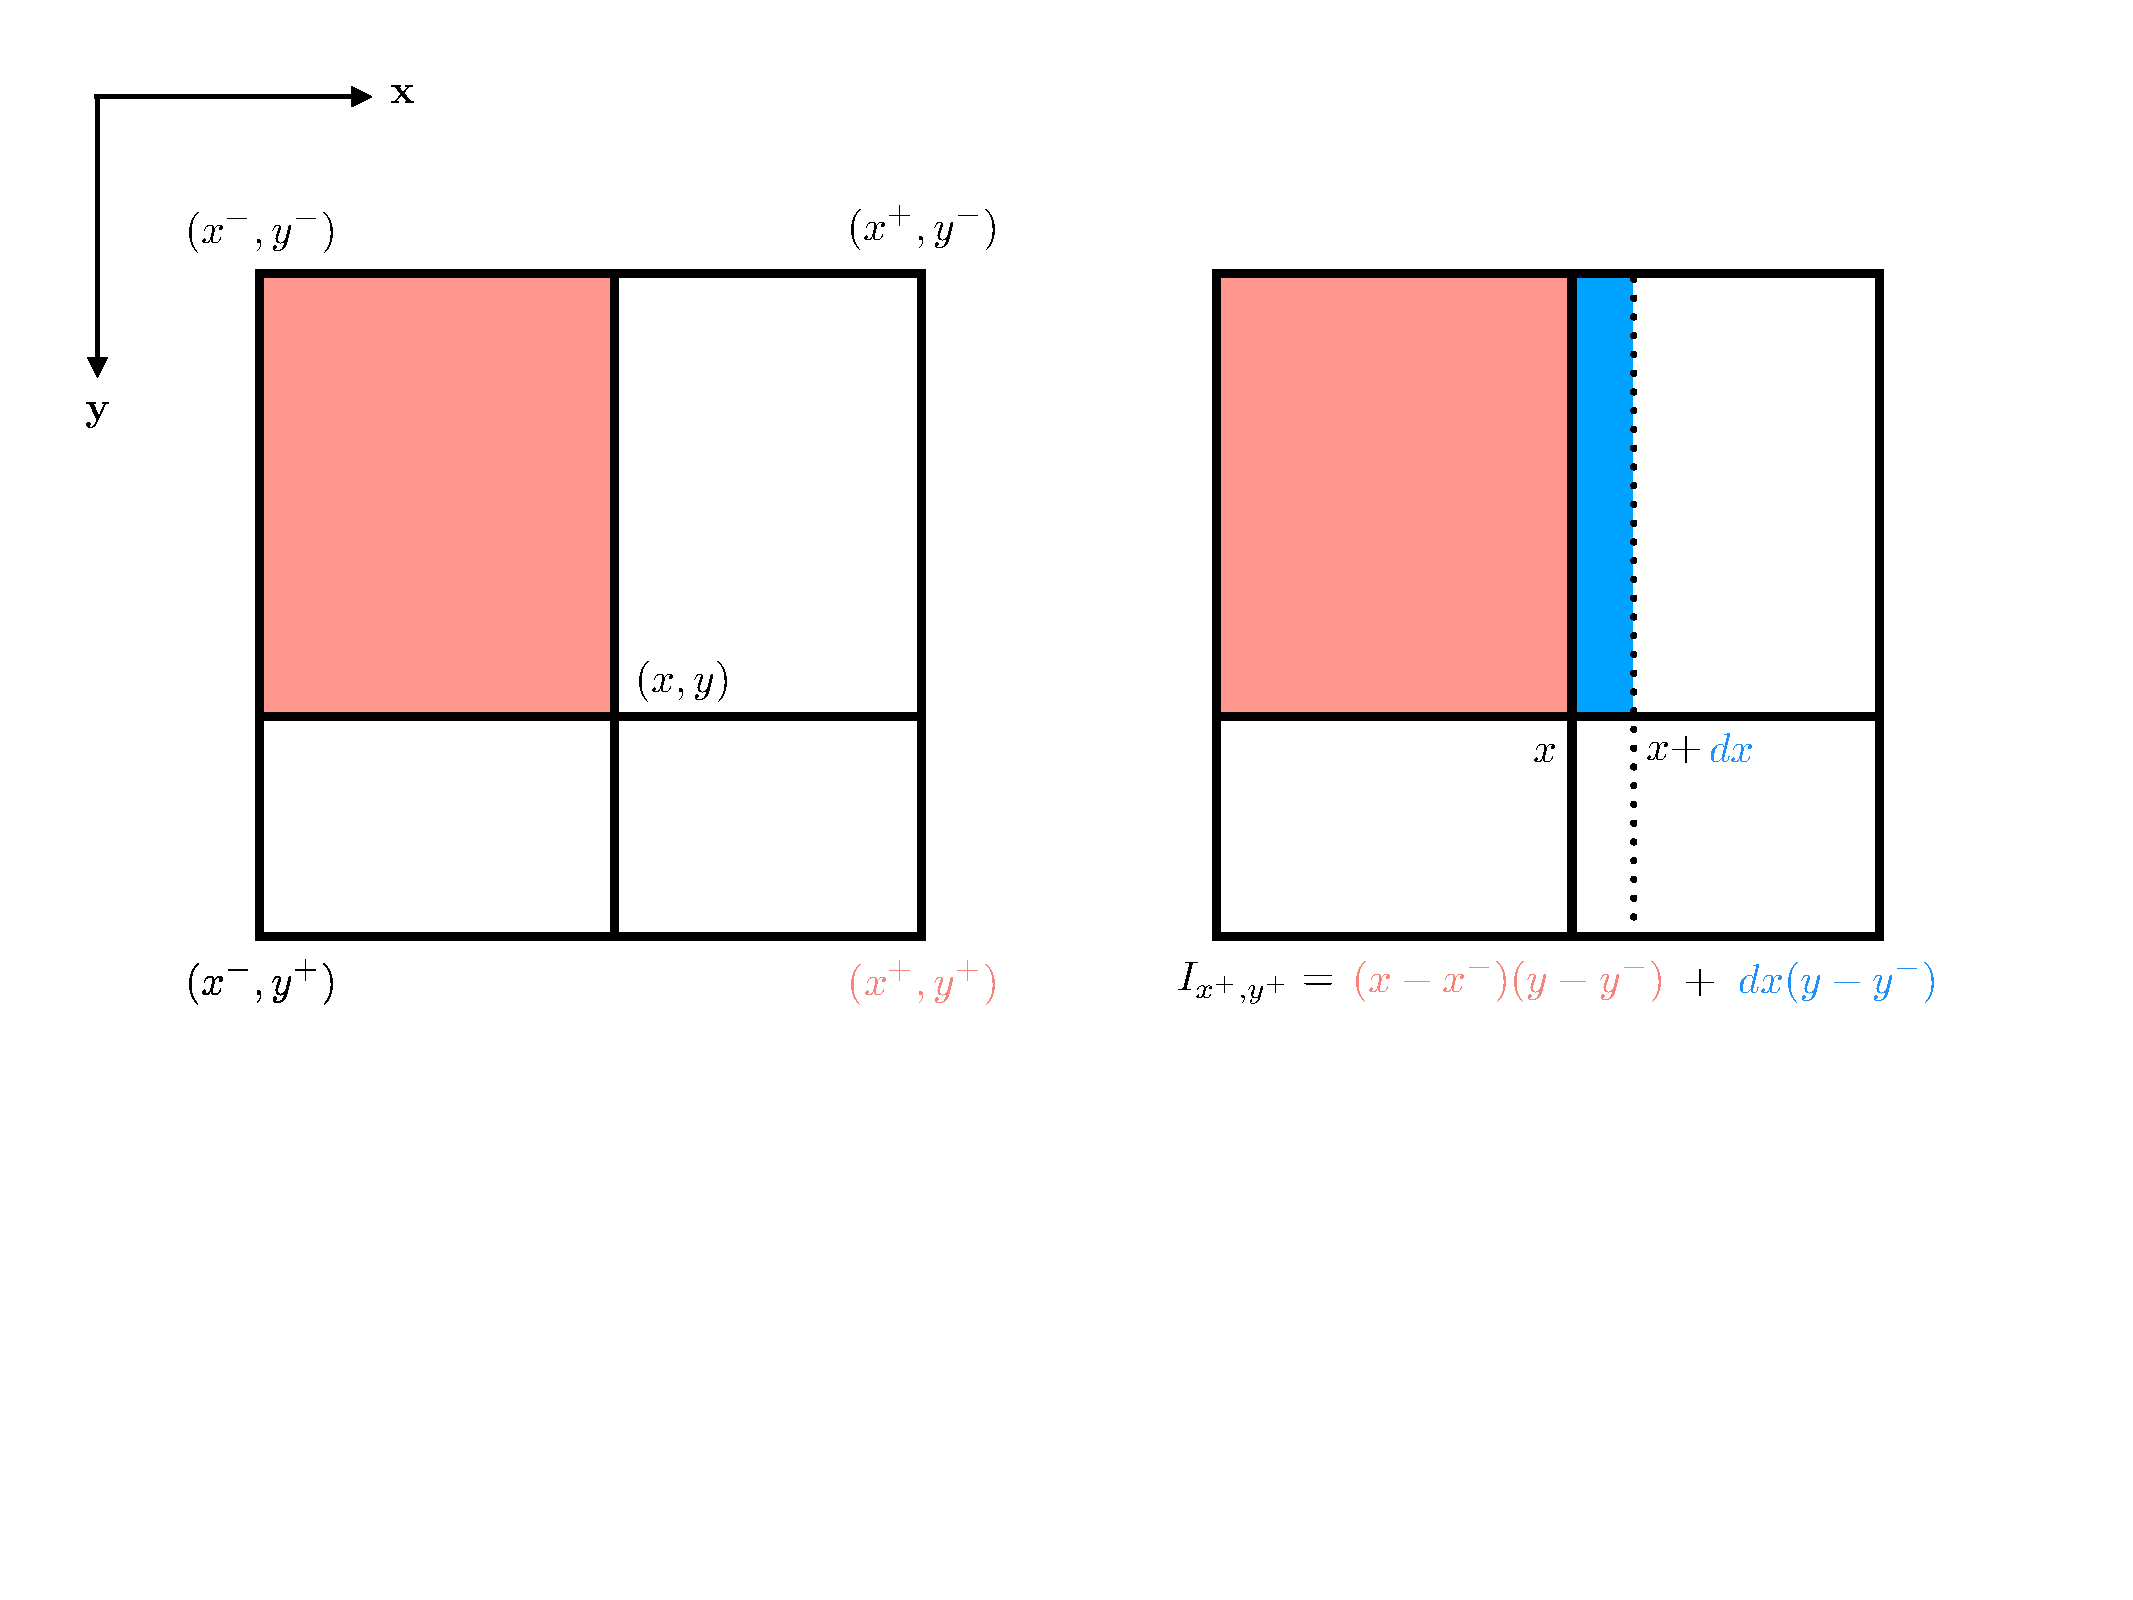
\includegraphics[trim={1cm 7cm 18cm 1cm},clip,width =
    \textwidth]{images/bi_voting.pdf} (a) The intensity at a pixel
    location is the area of the rectangle spanned by the opposite
    pixel and the event location
  \end{minipage}
  \hfill
  \begin{minipage}[t]{0.48\textwidth}
    \centering 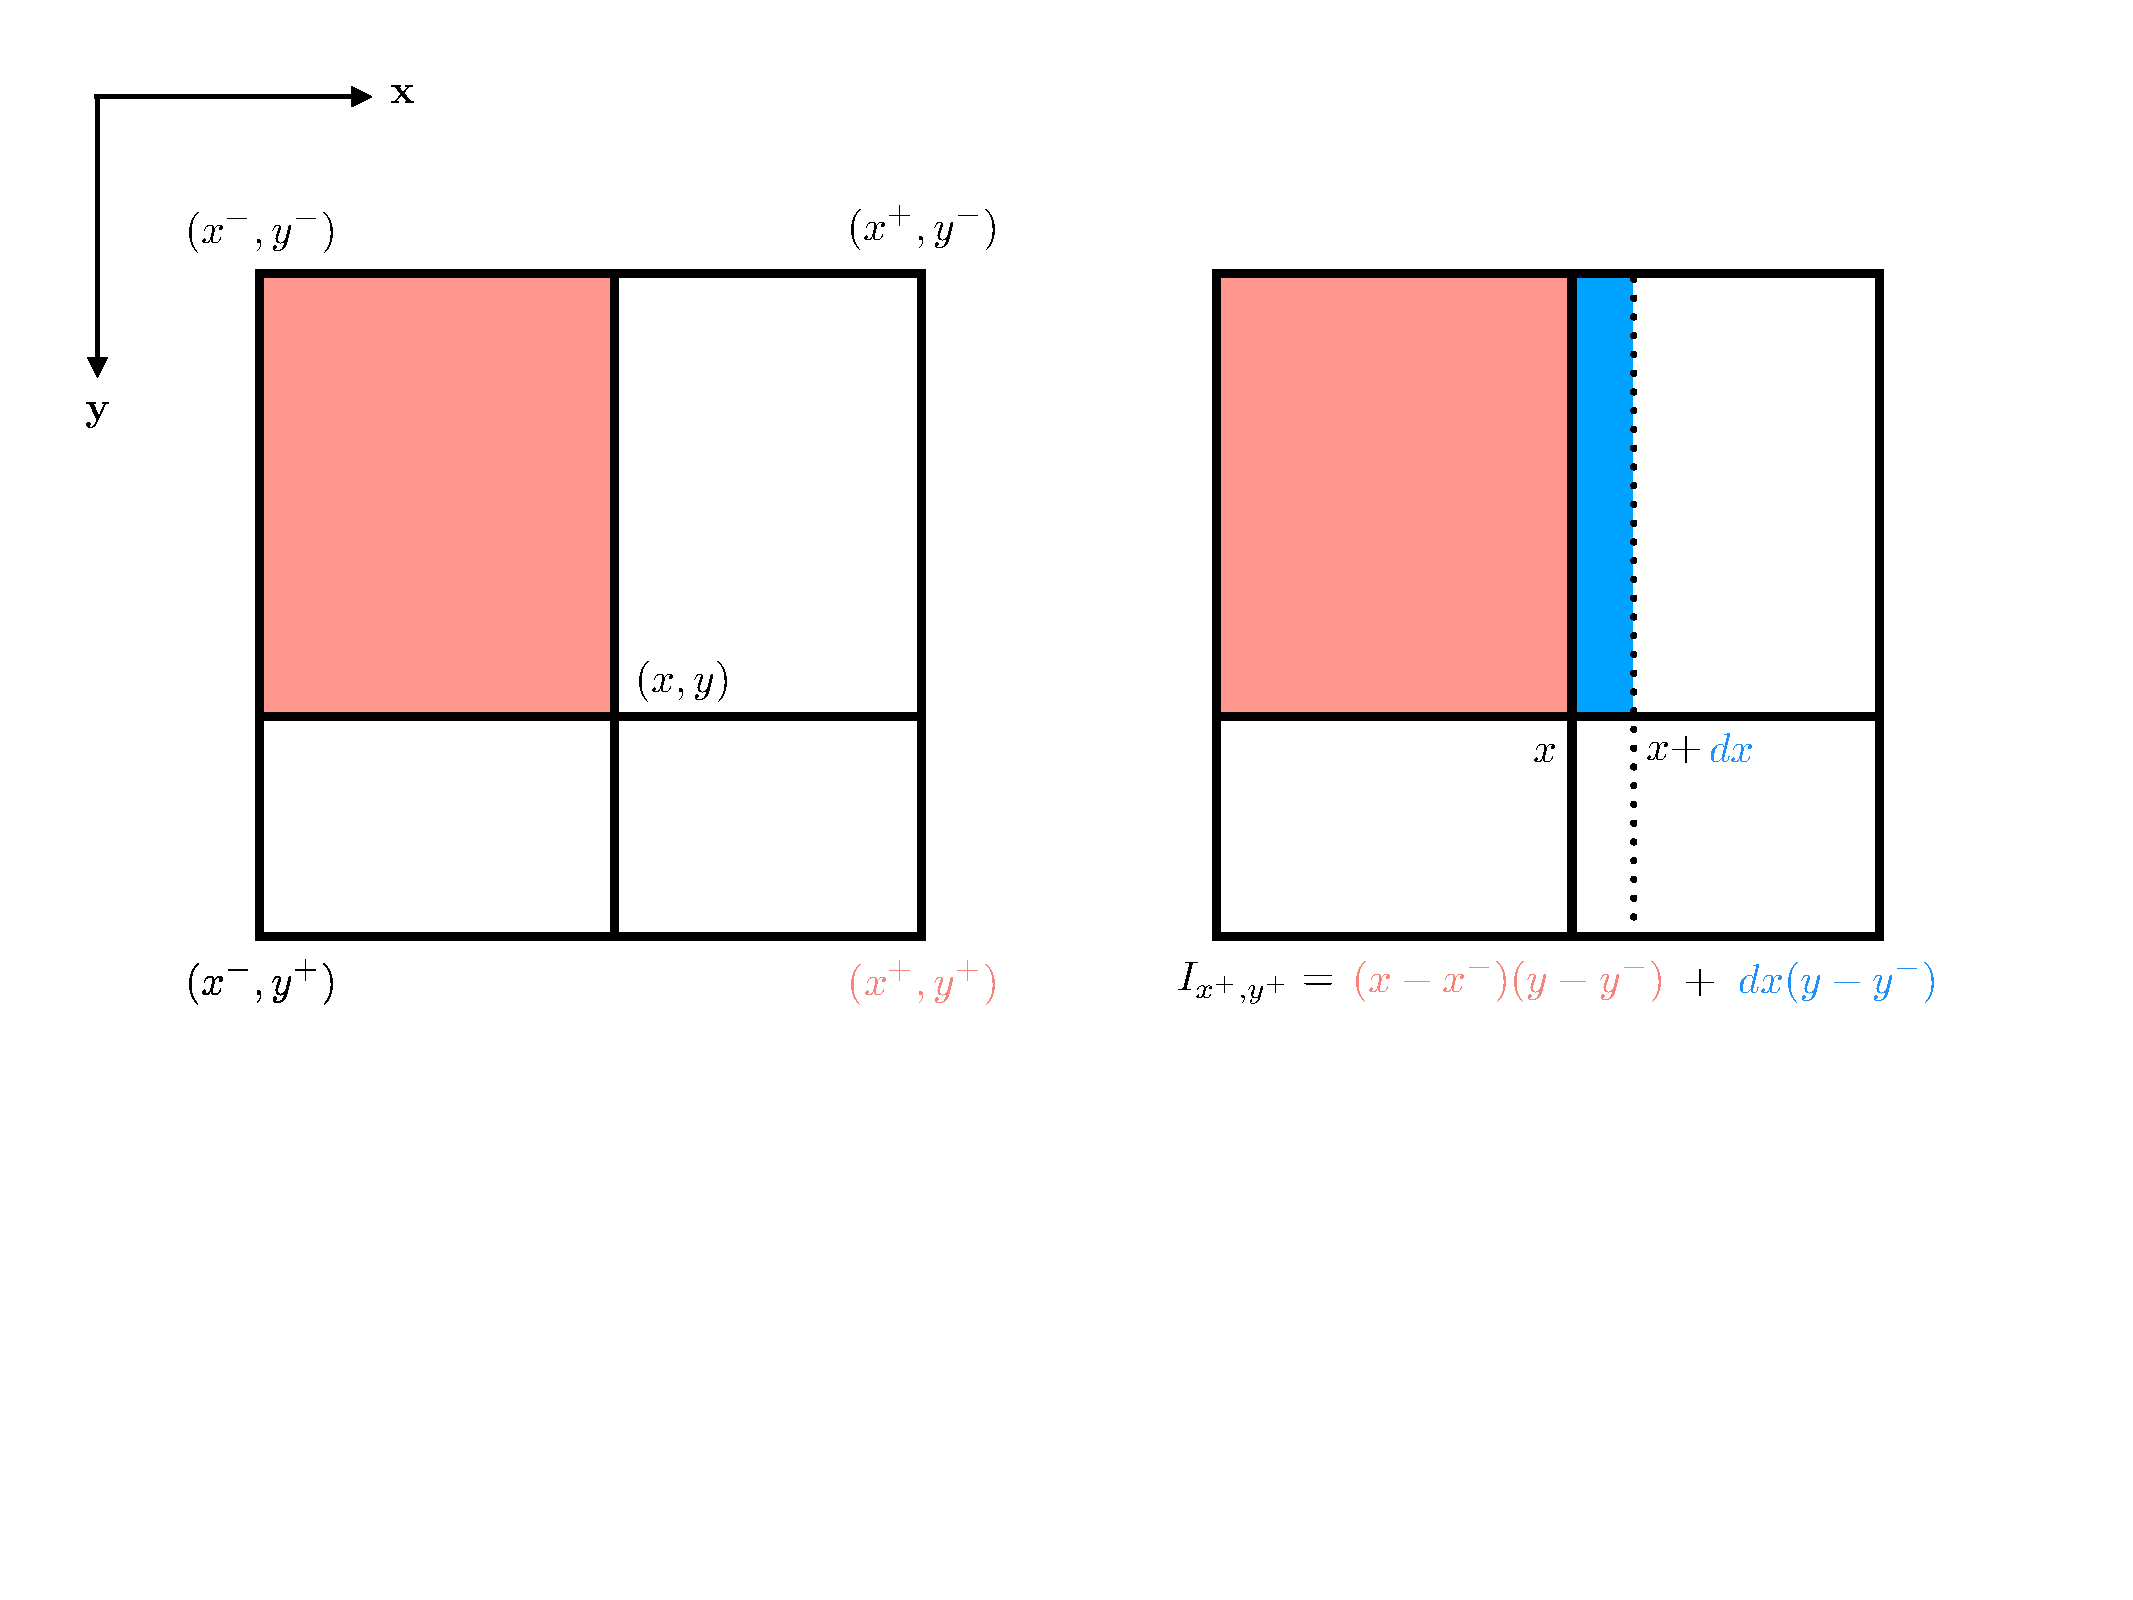
\includegraphics[trim={18cm 7cm 1cm 1cm},clip,width =
    \textwidth]{images/bi_voting.pdf} (b) Intensity change after an
    infinitesimal movement of the event
  \end{minipage}
  \caption{Bilear voting}
  \label{fig:bi_voting}
\end{figure}
The detailed algorithm for the evaluation of the Dirac delta as well
as its derivative is shown in algorithm.~\ref{alg:bi_voting}. The
behavior of the bilinear voting for derivatives is undefined when
$\vec{x}_k'$ locates exactly at a pixel location. However, the
possibility of this to happen is zero except when $t=0$, and can be
solved by simply discarding the event or disturbing with a small
random noise. When projecting back to the map, The author uses a
project matrix with different focal lengths than the ones in the
camera calibration matrix, so that there won't be event at integer
pixel locations after warping.
\begin{algorithm}
  \label{alg:bi_voting}
  \DontPrintSemicolon \SetAlgoLined \SetKwInOut{Input}{Input}
  \SetKwInOut{Output}{Output} \Input{A warped event
    $e'_k=\{x_k',y_k',t_k\}$} \Output{The \textit{Dirac delta}
    $\delta(\vec{x}-\vec{x}'_k)$ as well as its derivative
    $\frac{\partial\delta(\vec{x}-\vec{x}'_k)}{\partial\vec{x}'_k}$}
  \hrule\; Let\;
  $x^-=\lfloor x'_k\rfloor, x^+=\lceil x'_k\rceil,y^-=\lfloor
  y'_k\rfloor, y^+=\lceil y'_k\rceil$\; Then\;
  $\delta(x^--x'_k,y^--y'_k)=(x-x^+)(y-y^+)$\;
  $\delta(x^--x'_k,y^+-y'_k)=-(x-x^+)(y-y^-)$\;
  $\delta(x^+-x'_k,y^--y'_k)=-(x-x^-)(y-y^+)$\;
  $\delta(x^+-x'_k,y^+-y'_k)=(x-x^-)(y-y^-)$\;
  $\frac{\partial\delta(x^--x'_k,y^--y'_k)}{\partial
    x'_k}=y-y^+,\frac{\partial\delta(x^--x'_k,y^--y'_k)}{\partial
    y'_k}=x-x^+$\;
  $\frac{\partial\delta(x^--x'_k,y^+-y'_k)}{\partial
    x'_k}=-(y-y^-),\frac{\partial\delta(x^--x'_k,y^+-y'_k)}{\partial
    y'_k}=-(x-x^+)$\;
  $\frac{\partial\delta(x^+-x'_k,y^--y'_k)}{\partial
    x'_k}=-(y-y^+),\frac{\partial\delta(x^+-x'_k,y^--y'_k)}{\partial
    y'_k}=-(x-x^-)$\;
  $\frac{\partial\delta(x^+-x'_k,y^+-y'_k)}{\partial
    x'_k}=y-y^-,\frac{\partial\delta(x^+-x'_k,y^+-y'_k)}{\partial
    y'_k}=x-x^-$\;
  \caption{Bilinear Voting}
\end{algorithm}
\BlankLine
By linearity of the mean and the derivative, gaussian smoothing

However, a general nonlinear optimization is usually very hard,
especially at bundle adjustment stage he jacobian matrix only measures
the local grad
\cleardoublepage
\chapter{Datasheets}\label{sec:datasheets}

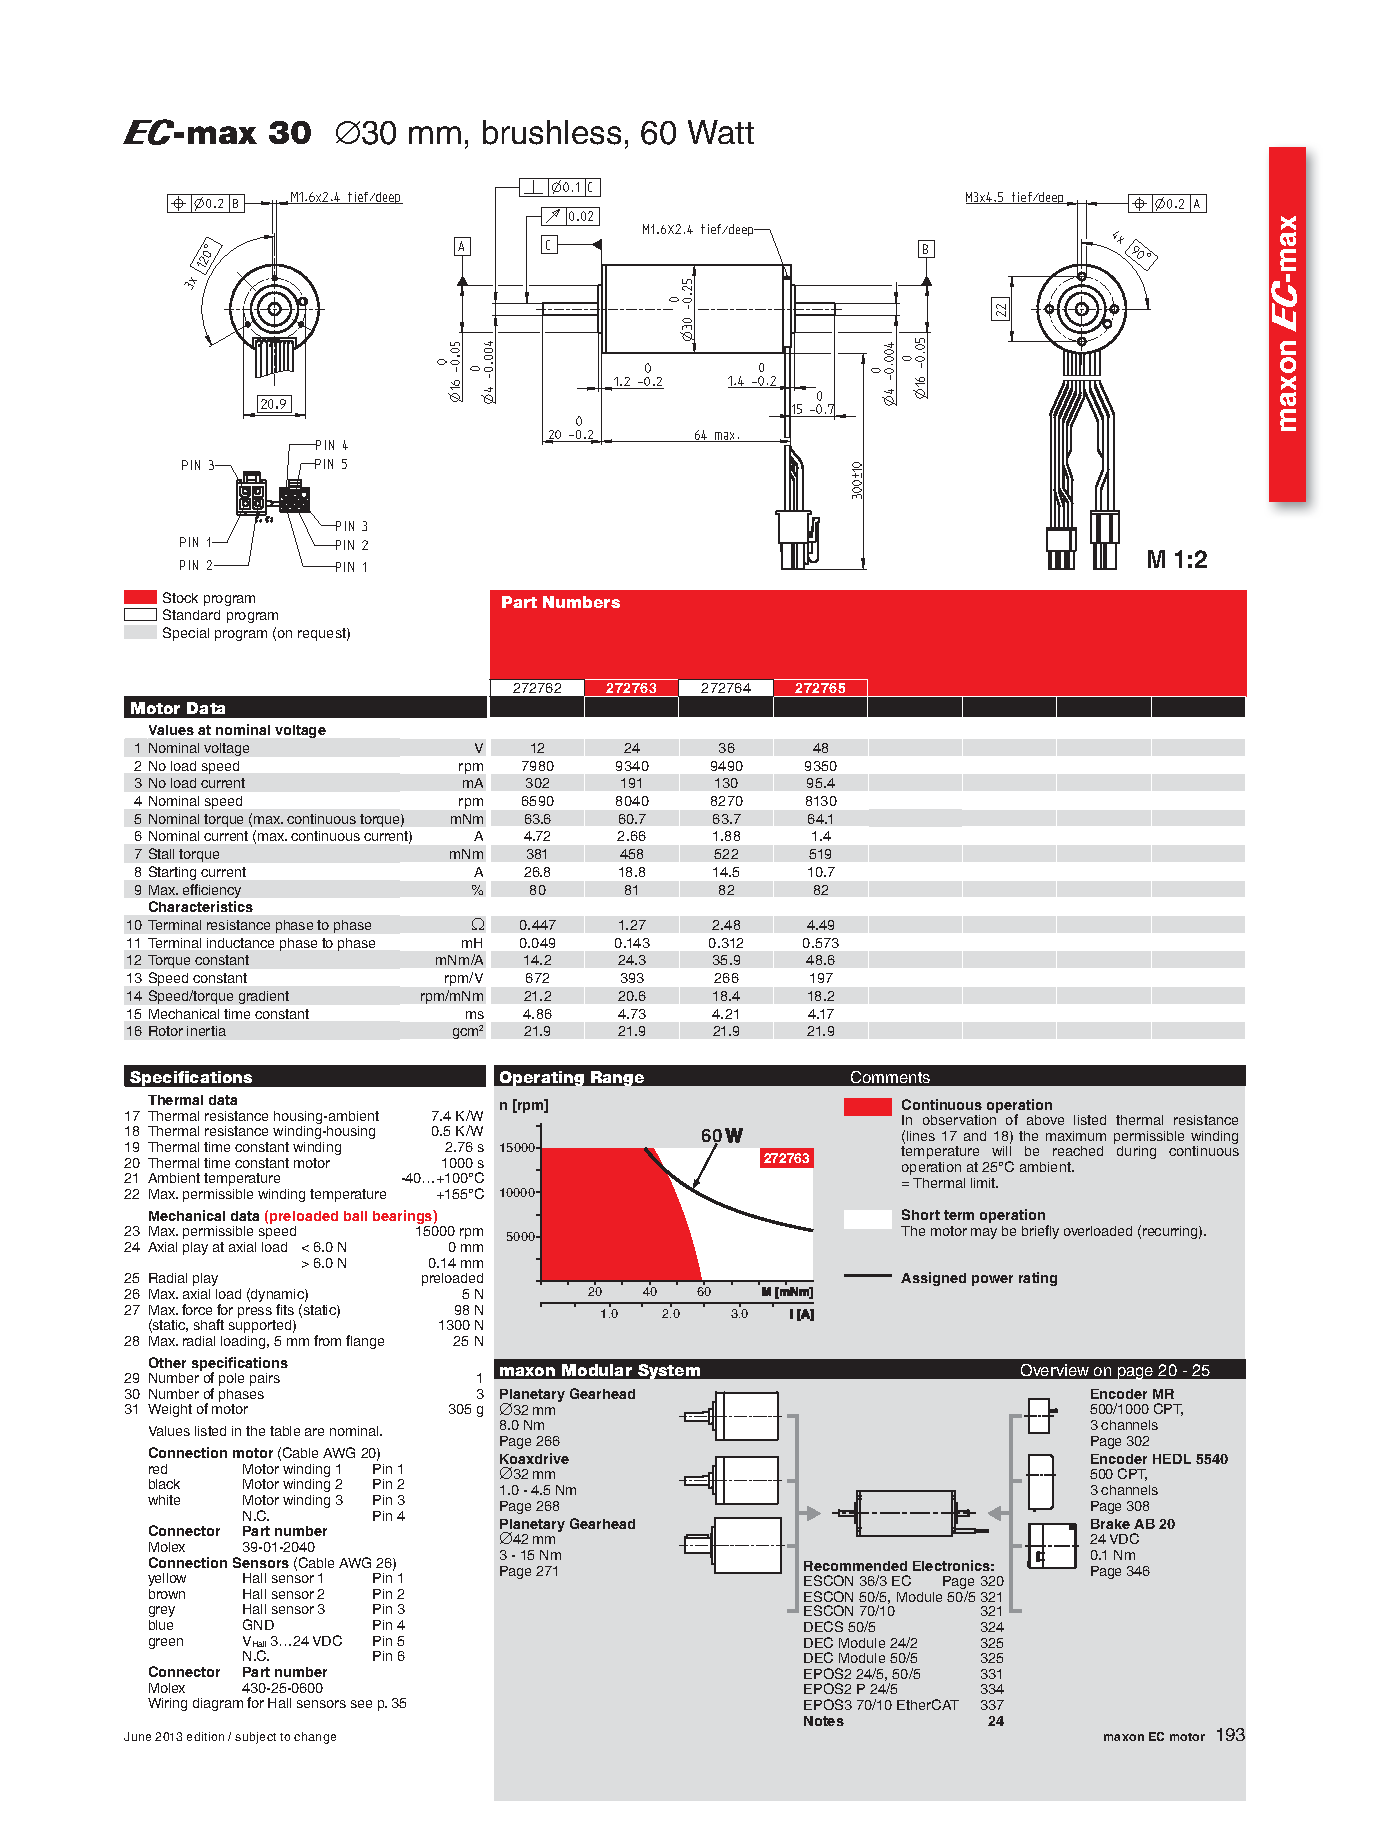
\includepdf[scale=0.75]{images/datasheets.pdf}

\end{document}
